\part{State of the Art}

%\part{Optimization}

\chapter{Optimization - Basic Concepts}

[[TODO: Ajouter quelques refs]]

Before starting to present the different categories of optimization, we would like to take some time to define what exactly optimization is.\\
In the more general way, optimizing is \emph{trying to find the best element among an element set}. When finding this best element is not trivial, we can rightfully talk of \emph{solving an optimization problem}. This seemingly simple definition implies in fact quite a lot.

First of all it requires a defined set of elements to choose from. As we will see, the topology of the set is of the utmost importance for choosing the way of solving the problem. This set of elements is often named the \emph{search space}, \emph{solution space} or \emph{domain}. In \enquote{simple} optimization problems, the search space can be simply defined by a set of elements (for example \{a,b,c\} or \ensuremath{\mathbb{R}}) associated with a set of \emph{constraints}. For large problems, the search space can be defined by calculus-heavy equations, empirical models, complex algorithms ... or even a mix of all of the above.

\definition{Search space}{the set containing all the possible candidates for the optimization problem.}

While we said that the search space can be defined by a set of constraints, it is often more convenient to express the constraints separately. For example, if the search space of an optimization problem is defined over all the real numbers lower than 2, instead of defining the search space as [-\(\infty\) : 2], it will usually be refereed as \(\mathbb{R}\), with the added constraint \(x < 2\). Usually we say the problem to be \emph{subject to (s. t.)} the constraint \(x < 2\).\\
In theory these two formulations should be equivalent. In practice however, these constraints are often the result of a real-world concern, and thus subject to some inherent imprecision. Let us imagine an optimization problem defined by an engineer trying to design an aircraft. Among the constraints defined by the engineers, the aircraft weight must be lower or equal to 40t. Does it means that a solution for which the weight of the aircraft would be 40t \emph{and 200g} would be completely unacceptable? Obviously not, the designer may be willing to accept some concessions in regard of the violation of this constraint. In engineering design, this is a common situation, and making these constraints explicit can be advantageous.

Since we want to find the best element of this solution space, we have to determine what makes an element better than another. Usually, the possible solutions are compared through a specific function called the \emph{objective function}. Some alternate names are \emph{criterion} or \emph{cost function}. The best element would be the one for which the objective function returns a minimal (or alternatively, maximal\footnote{Obviously we sometimes want to find the \emph{maximal} value that is solution of a problem, however minimizing f(x) is equivalent to maximizing (-f(x)). So maximization problems can be expressed as minimization problems, and vice-versa. Traditionally, optimization problems are often expressed in the terms of finding a \emph{minimal} value since the two possibilities are equivalents.}) value. It should be noted that it is possible for a problem to admit several equivalent solutions in regard of the objective function.

\definition{Objective function}{a function defined over the search space of the optimization problems, expressing the aim of a stakeholder for this problem.}

When the search space is very large, or its topology is complicated, it can be really long or difficult to find the best solution and, more important, to be sure that the solution is the best. In fact, in these problems, the only way to find the best solution with certainty is an exhaustive exploration of the search space. Since it can be very costly regarding time and computation, instead of finding the best solution, we settle for the best known, which is considered to be \enquote{good enough}, for example because this solution is the best of its neighborhood for a subset of the search space. The absolute best solution is called the \emph{global optimum}, while the best known solution is called a \emph{local optimum}. In a similar fashion, methods which try to find the global solution are said to be \emph{global optimization methods}, where methods which are driven by local optima are said to be \emph{local optimization methods}.

\definition{Optimizing}{finding an element of the search space that minimizes (or maximizes) the value of the objective-function}

\begin{figure}
\centering
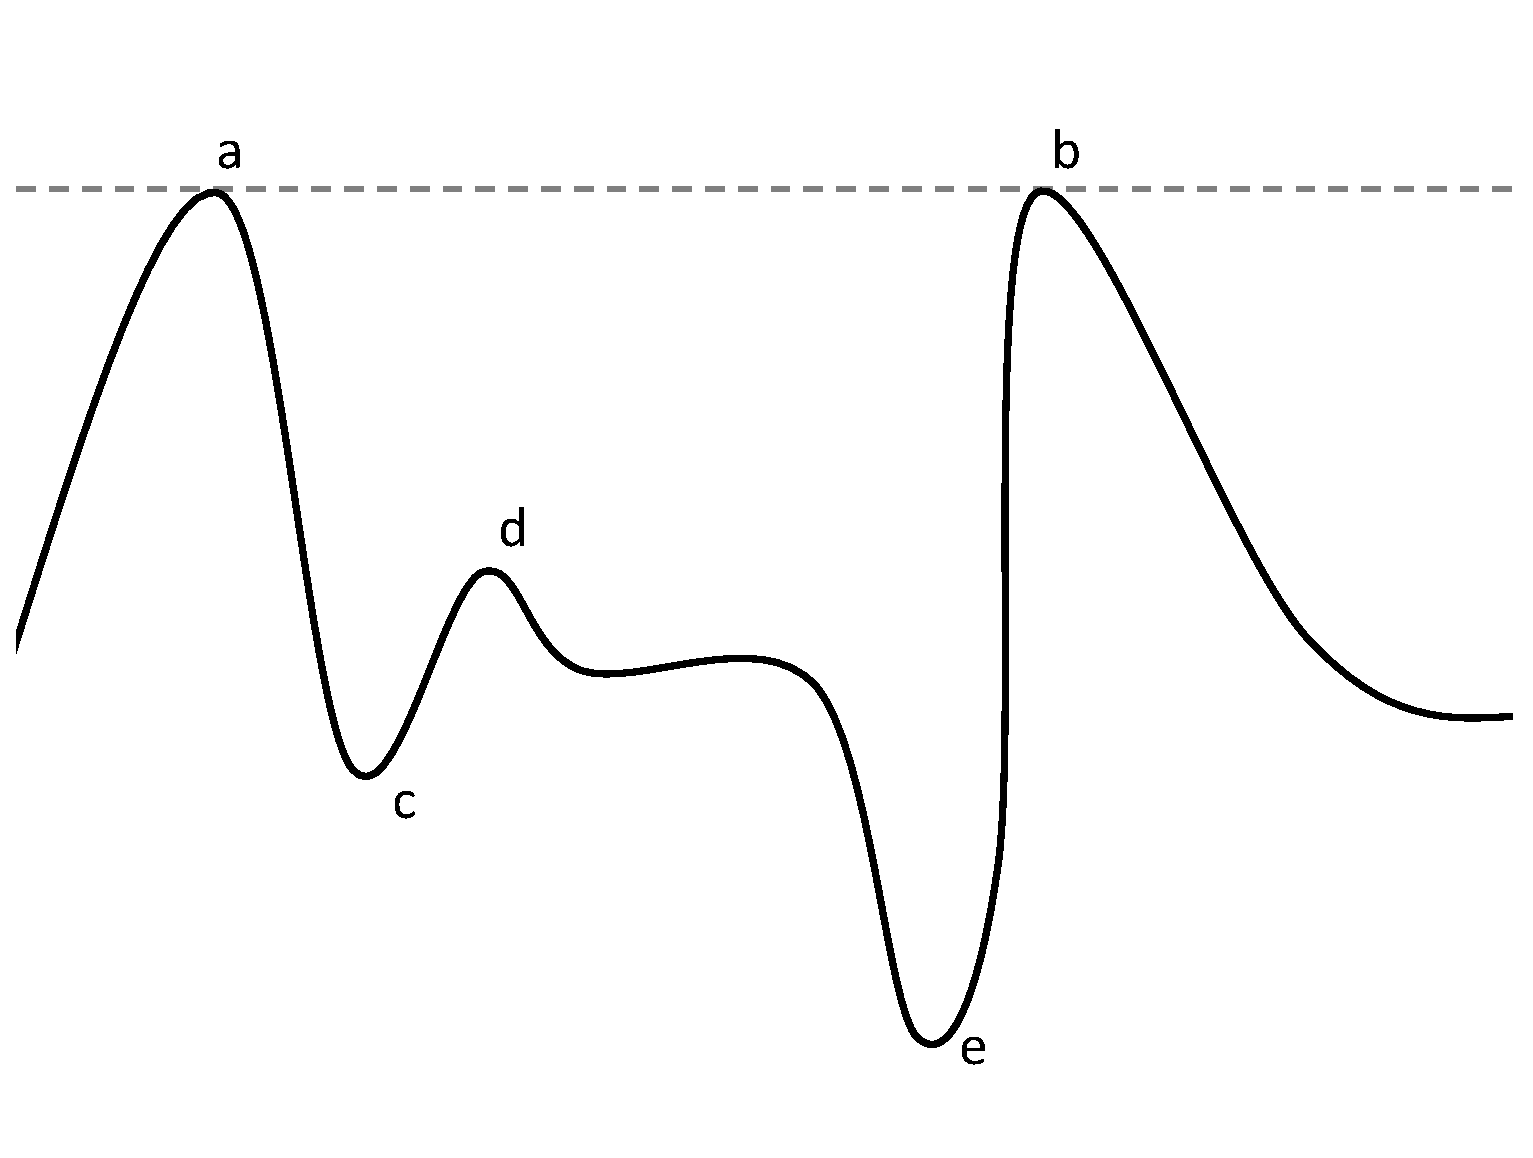
\includegraphics[width=0.4\paperwidth]{searchSpace}
\caption{Examples of local and global optima - $a$ and $b$ are global maxima, $c$ is a local minimum, $d$ is a local maximum and $e$ is a global minimum.}
\label{localAndGlobalOptims}
\end{figure}

In figure \ref{localAndGlobalOptims}, we can see different examples of global and local optima. The points labeled \emph{a} and \emph{b} are both global maxima, as they have the same value. The points
\emph{c} and \emph{d} are respectively local minimum and maximum, while \emph{e} is the global minimum.

From all the preceding, we can provide the minimal formulation of an optimization problem as follows:

\begin{align*}
\text{minimize } &f(x) \\
\text{subject to } &(x \in S)
\end{align*}
Where \emph{S} is the problem search space and \emph{f(x)} the objective function.

\section{Continuous versus Discrete Optimization}

Before going further into details, we must make an important distinction between \emph{continuous} optimization (also called \emph{numerical} optimization) and \emph{combinatorial} optimization. The difference between the two categories concerns the definition domain of the variables, and consequently the nature of the search space. For combinatorial optimization, the variables can only take a finite number of different values (their definition domain is a finite and enumerable set), while the definition domain of continuous optimization problem variables is, as the name implies, continuous (thus the variable can take an infinite number of values).

This distinction has a profound impact on the nature of the problems. While the search space of a combinatorial optimization problem is finite, a continuous optimization problem can have an infinite number of potential solutions. Interestingly, this distinction does not implies that continuous optimization problems are inherently harder to solve than discrete ones. While combinatorial optimization problems can be NP-complete in the general case, some continuous optimization problems can easily be solved in polynomial time (even large ones). This surprising properties comes from the fact that complexity of combinatorial optimization problem comes from the difficulty to efficiently explore the different possibles variables states combinations, whereas for continuous optimization, the difficulty comes more from the shape of the search space. In simple continuous optimization problems, the search space will be very regular, and the optimum easy to find, while optimization problems with complicated, \enquote{chaotic} search spaces will be much more difficult to solve.

For the sake of completeness, let us add that there exists an optimization field which is at the border between continuous and combinatorial optimization, named \emph{Integer programming}\footnote{in this context, \enquote{programming} must not be mistaken with computer programming but be understood as a synonym for \enquote{optimization}. This peculiar use of the word comes from the historical origins of the optimization field.}, in which the variables are must take integer values but are not restricted to a bounded definition domain (making their definition set countable but infinite). An extension of these problems are \emph{mixed-integer programs}, where some of the variables are restricted to integer values and some are not. For more informations on integer programming, the reader can refers to \cite{schrijver1998theory}. Integer programming an combinatorial optimization are sometimes regrouped under the \emph{discrete optimization} category. The terms \emph{combinatorial} and \emph{discrete} seems to often be used somewhat interchangeably.

In the context of this thesis, we will concern ourselves more specifically with continuous optimization. For more works concerning combinatorial optimization problems from a multi-agents systems perspective see [[REFS]].

\section{No Free Lunch Theorem}

The No Free Lunch (NFL) Theorems for optimization are important results in the field, formalized by Wolpert and Macready \cite{585893}. The basic idea behind these theorems is that no optimization method outperforms the others when regarding the class of all the possible problems or, as the authors themselves say:
\begin{quote}
\enquote{any two algorithms are equivalent when their performance is averaged across all possible problems.}
\end{quote}
If an algorithm outperforms another on certain types of optimization problems, there must be others classes of problems where this algorithm performs worse.

The NFL theorems are based on several assumptions:
\begin{itemize}

\item the search space is finite,

\item the optimization algorithms never re-evaluate the same point.

\end{itemize}

The first assumption limits the scope of NFL theorems to the realm of combinatorial optimization, as continuous optimization problems contain by nature an infinity of elements. Indeed, it has been shown that, in the context of continuous optimization, free lunches were indeed possible \cite{Auger-s00453-008-9244-5} (but possibly at the cost of very big memory footprint). Thus this result does not impact directly the scope of this work, but we believe that it is still a good illustration of one of the main problematics of the optimization research field, which is that one must often compromise between universality and efficiency. Even in the context of continuous optimization, where the existence of free lunches has been demonstrated, it is probable that we will never find a be-all and end-all optimization technique. This point is for example discussed in \cite{Doe05}.

One example which can be connected to the NFL is the compromise between exploration and exploitation. Basically, an optimization method must often make a compromise between using the previous results to converge toward a region of the search space and exploring the remaining of the search space to find a better region.
For example: some gradient-based methods will use the evaluated points to converge toward a local optimum, but can miss a better solution as they explored the search space insufficiently. On the opposite, some others methods can make a thorough exploration of the search space (by partitioning or random drawing points), but will be slow to converge towards the exact optimum.
It is often possible to parametrize the method to tune the compromise between exploration and exploitation regarding the nature of the problem at hand but a relevant parametrization requires a sufficient knowledge of the properties of the problem and therefore a parametrized method is efficient only for a specific problem.

Of course, the NFL theorems consider \emph{all the possible objective-functions}. One could argue that \enquote{interesting} problems (at least from en engineering point of view) are not distributed evenly over such a space, but correspond to a subset for which some optimization methods are more efficient than others. This is why optimization as a scientific research domain makes sense. 

This distinction has been formalized by differentiating \emph{incompressible} from \emph{compressible} objective-functions. Incompressible objective-functions are random and it is thus impossible to develop an optimization method to find the solution efficiently, since good and bad values are randomly distributed. Of course, such \enquote{impossible} objectives function make for the major part of all the possible objective-functions \cite{English:3-540-45356-3_7}.
As we said, the set of \enquote{interesting} objective-functions, or even the set of real-world related ones is much much more restrained. And for this specific category, some optimizers are better than others. 
However, as we will see in the next sections, the variety of \enquote{interesting} optimization problems is still important enough to have resulted in a great variety of specific optimization techniques.

One consequence of the NFL is that selecting an efficient optimization method for a given problem requires to have at least a minimum insight on the properties of the problem. No algorithm can be deemed most efficient for the general case.

On a side note, it can be added that, in addition to the case of continuous optimization, the possible existence of free lunches has been demonstrated for coevolutionary \cite{1545946} as well as multiobjective optimization \cite{1299403}.

\chapter{Continuous Optimization}

As we have seen at the end of the last chapter, optimization methods have to make various compromises regarding applicability versus efficiency.  A great variety of methods exit in the literature, from generic methods applicable to a great variety of optimization problems to very specialized methods designed to be efficient in a specific context. These methods can be categorized by the type of problems they aim to solve or some inherent properties of the method.

Some possible criteria to discriminate based on the type of problem:
\begin{itemize}
\item can we obtain derivatives of the functions defined in the problem?
\item is the problem linear (or possibly quadratic)?
\item is the problem convex?
\end{itemize}

For the method in itself:
\begin{itemize}
\item is the method able to take constraints into account?
\item does the method provide a global solution or a local one?
\item is the method deterministic or stochastic?
\end{itemize}

Based on the shape of the search space and our requirements regarding the method, we will try to choose the most adequate optimization method. As always, the more information known regarding the problem, the more we would be able to select a specialized method with a great efficiency. If very few information is known, it could be necessary to use black-box optimization methods, that is methods that do not make any assumption regarding the nature of the problem. These techniques can suffice in themselves to get a good-enough result, or can be used as a prelude of more specialized techniques if enough information is gathered.

A rough proposal of organization of the different types of continuous optimization can be seen in \ref{numerical_optim_tree}.

\begin{figure}
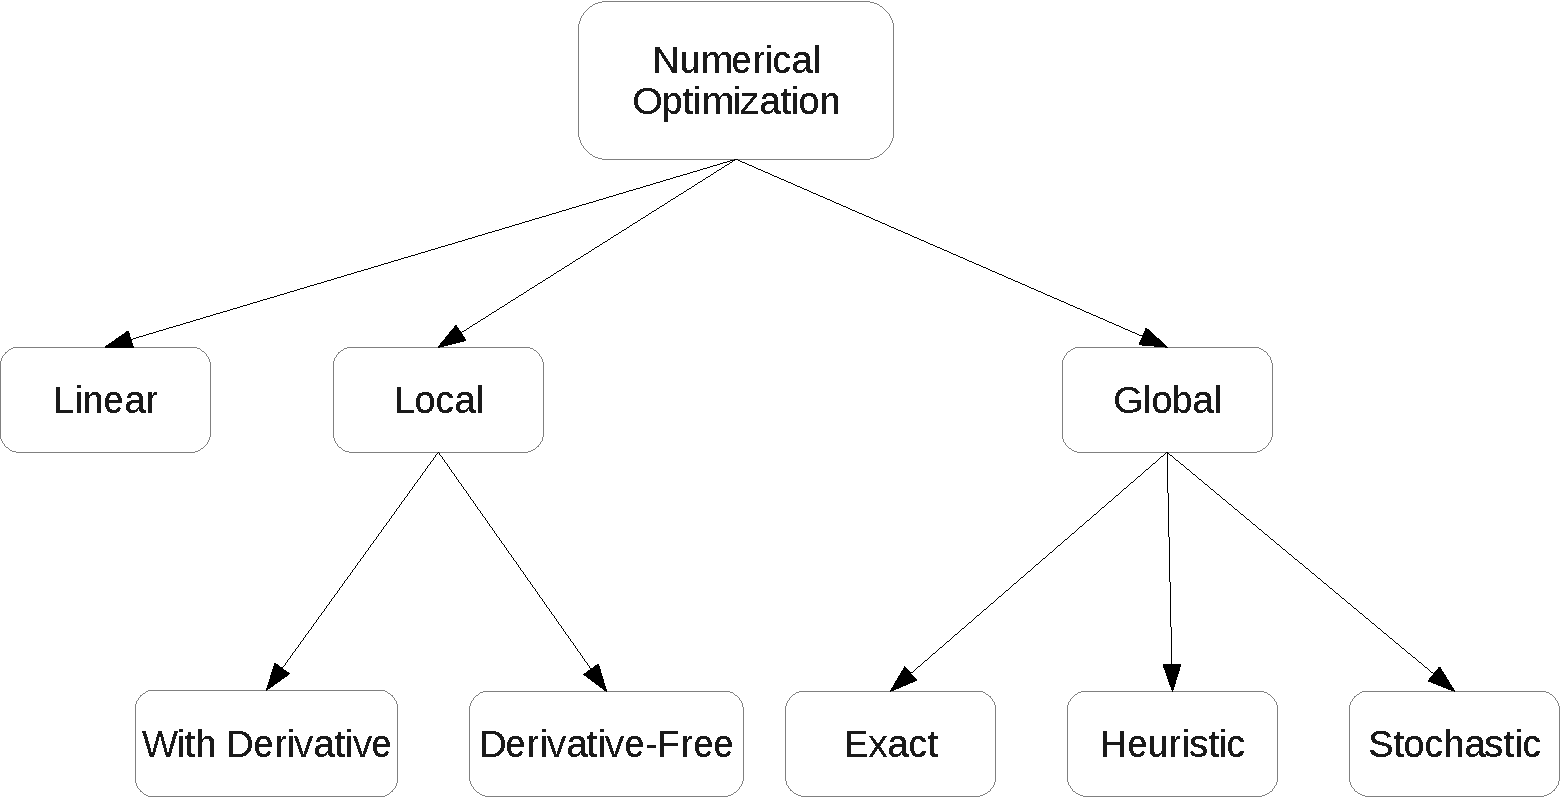
\includegraphics[width=\textwidth]{numerical_optim-crop}
\caption{Types of continuous optimization methods}
\label{numerical_optim_tree}
\end{figure}

Presenting all the continuous optimization techniques would be far outside the scope of this work. In this part we will focus on presenting briefly the different optimization categories we identified in figure \ref{numerical_optim_tree}. We will reference some of the most representatives techniques to illustrate this presentation, but without going too much into the details of the techniques.

\section{Linear Optimization}\label{linear_optim}

Linear optimization focuses on the solving of problems where the objective-function and constraints are linear (that is, $f(x+y) = f(x)+f(y)$ and $f(ax) = af(x)$) and the search space convex.

A \emph{convex} search space is a set where all the lines segments linking the points of the set are fully contained inside the set (if it is not the case, the set is said to be \emph{concave}). An illustration of the difference between convex and concave search spaces is shown on \figurename{} \ref{convexVSconcave}.

\begin{figure}
\centering
	\begin{subfigure}{0.35\textwidth}
		\centering
		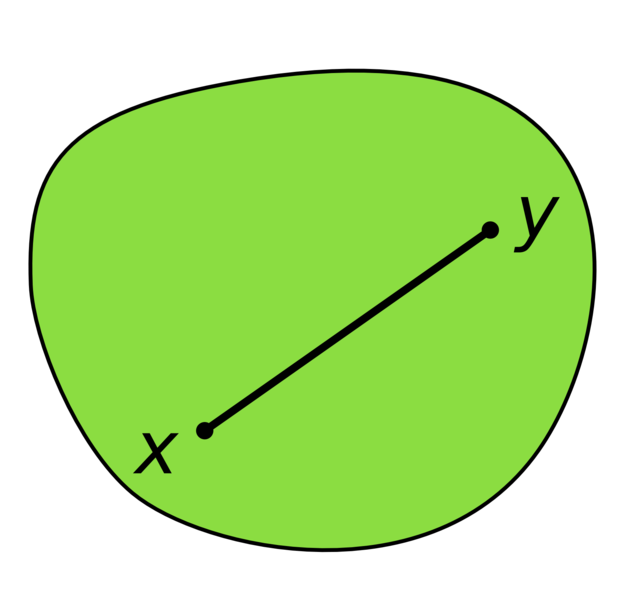
\includegraphics[width=\textwidth]{Convex_polygon_illustration1}
		\caption{Convex search space}\label{convexVSconcave:conc}
	\end{subfigure}
  	\begin{subfigure}{0.35\textwidth}
		\centering
		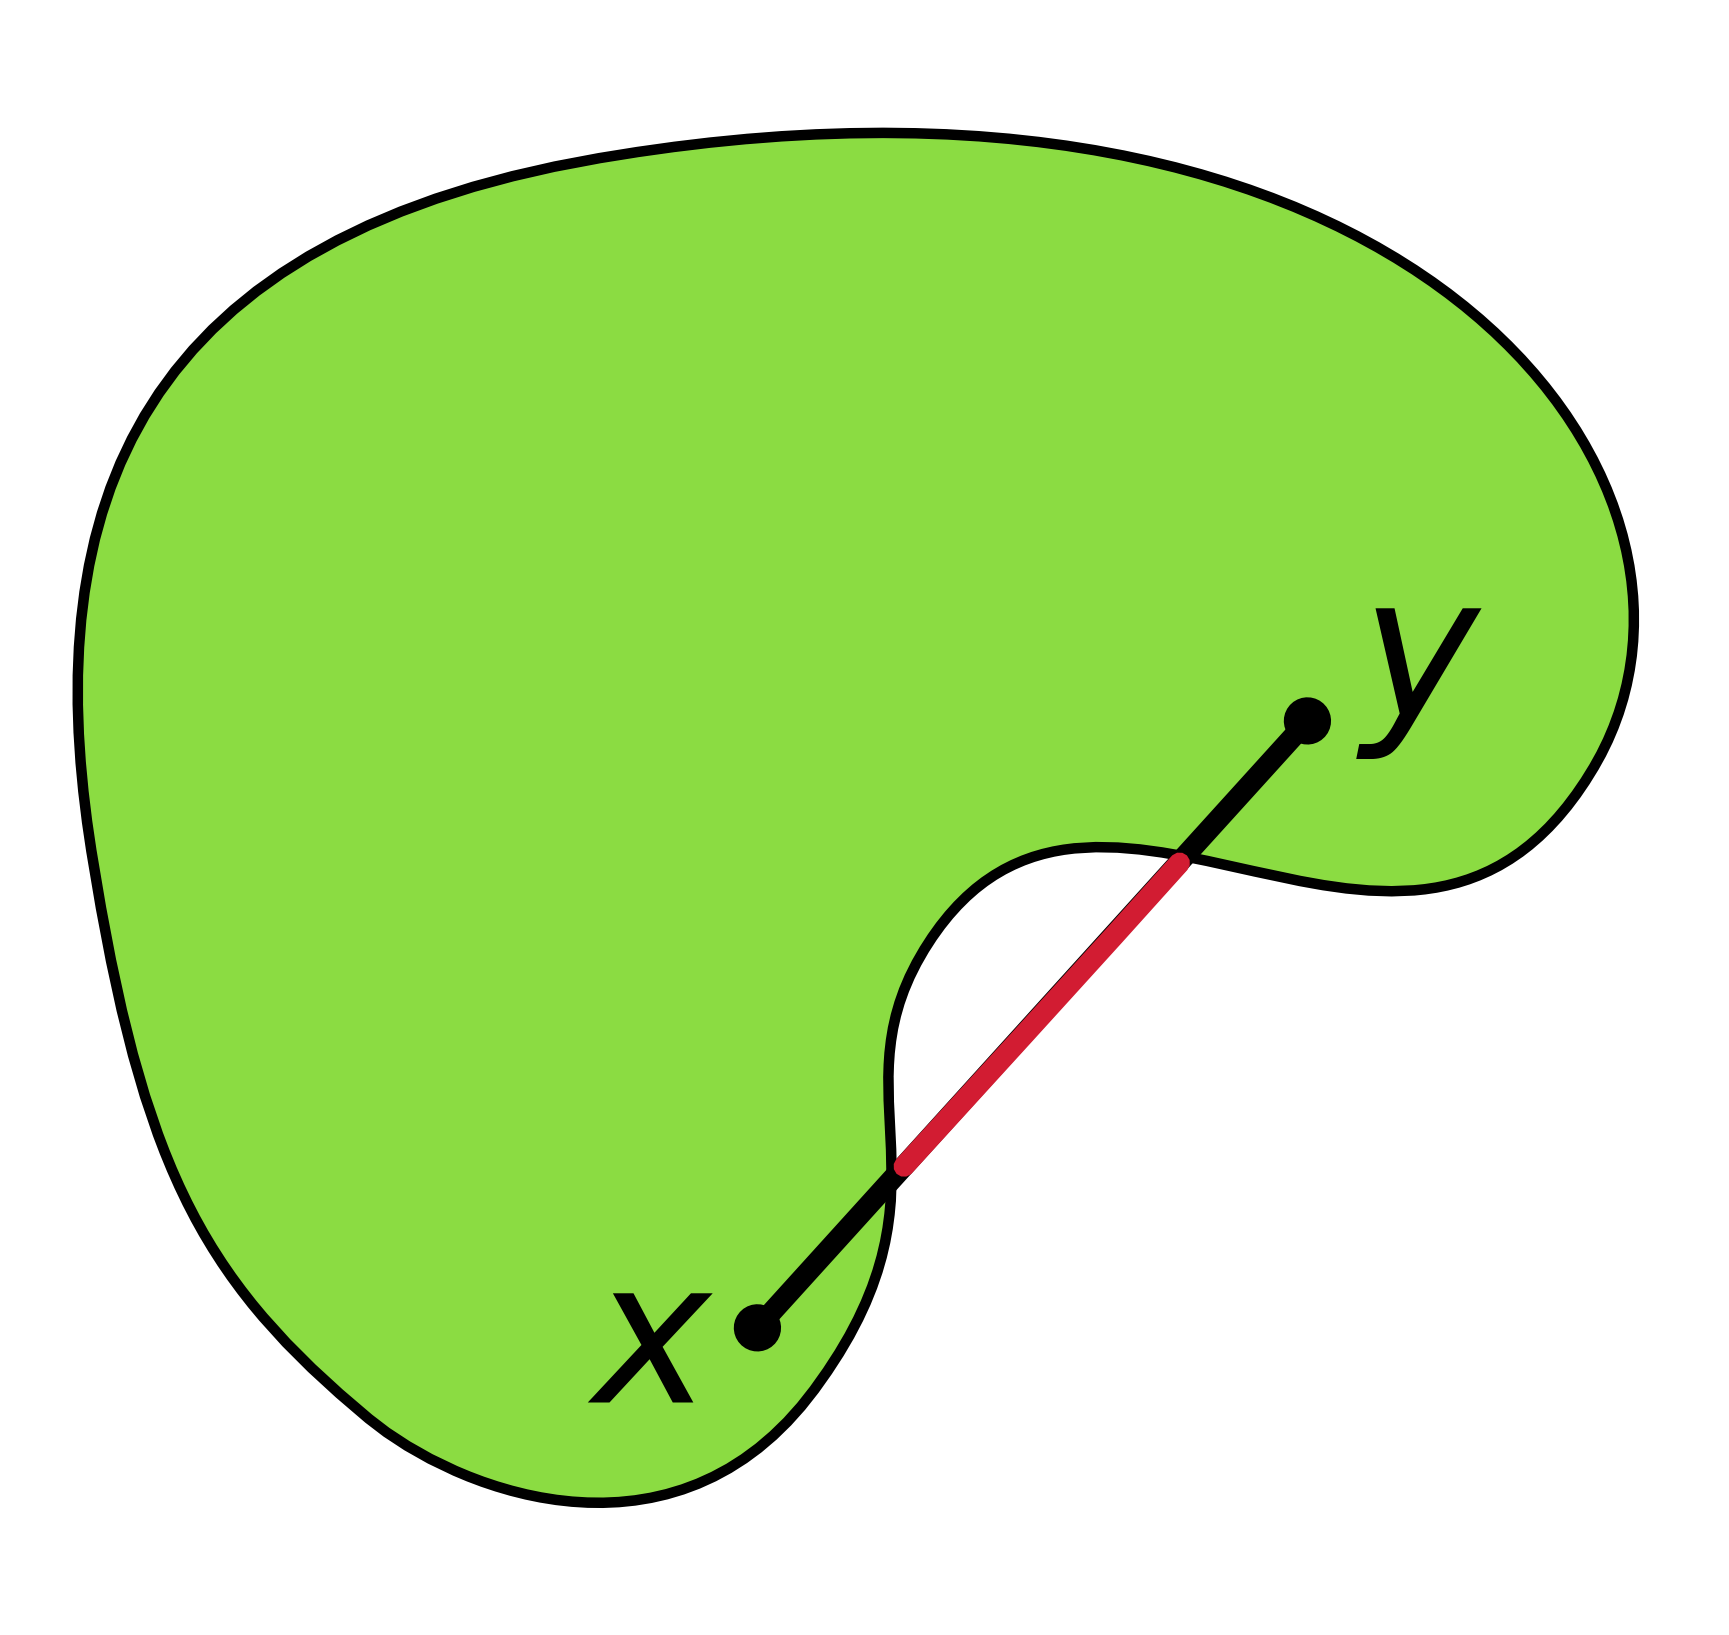
\includegraphics[width=\textwidth]{Convex_polygon_illustration2}
		\caption{Concave search space}\label{convexVSconcave:conv}
	\end{subfigure}
	
	\caption{Convex and concave search spaces (from \href{http://commons.wikimedia.org/wiki/Category:Files_by_User:Oleg_Alexandrov_from_en.wikipedia}{Oleg Alexandrov})}
	\label{convexVSconcave}

\end{figure}

A linear problem with $n$ variables and $m$ constraints can be expressed as:
\begin{align*}
\text{min } & a_1x_1 + a_2x_2... + a_nx_n\\
\text{subject to } &x_i \geq 0, \forall i \in 0,n\\
&a_{11}x_1 + a_{12}x_2 + ... + a_{1n}x_n + b_1 \geq 0\\
&...\\
&a_{m1}x_1 + a_{m2}x_2 + ... + a_{mn}x_n + b_m \geq 0
\end{align*}

This kind of problem is the most basic one. The most well-known method to solve linear problems is the Simplex algorithm \cite{dantzig1998linear}, published by Dantzig in 1947 (based on the work of Leonid Kantorovich). The Simplex algorithm is considered to be the first formal algorithm to solve a continuous optimization problem and to be one of the founding works of the field.

The basic idea of the simplex algorithm is that the solution space is the convex polyhedron, and the optimal solution is necessarily on one of its vertices. Another property is that a vertex which is not the optimal solution will have at least an edge leading toward a better vertex.
The simplex algorithm starts on one of the vertices, and tries to follow an edge to a vertex which improves the objective-function. The algorithm iterates until it has found a vertex with no edge leading toward a better point (the optimal solution) or until it reaches an unbound edge (in this case the problem is not bounded).

While the simplex algorithm is considered to be very efficient for most cases, some alternatives have been proposed. The most noteworthy is the interior point method and its derivatives. Contrary to the simplex method, this method actually traverses the interior of the solution space (hence its name). The original method proposed by Karmarkar \cite{Karmarkar:1984:NPA:800057.808695} travels through the search space by iteratively finding the best solution over a restricted region delimited by a sphere around the current point.

\section{Local Methods}

Unconstrained local optimization methods concentrate on finding local optima either because the search space is too big or to complex to find a global optimum in a reasonable time, or because we prefer to quickly find a good enough solution.
 Moreover, if the objective-function is convex, the local optimum is also the global optimum, in this context local methods can be an easy mean to obtain the best solution.

\subsection{Using Derivatives}

If the derivatives are available, it is possible to propose very efficient optimization techniques to converge toward a local optimum.

In some cases, even if the derivatives are not available, it is possible to obtain an approximation of the derivatives using for example a finite difference method. The basic idea of finite difference is to estimate the derivative from the ratio between the variation of the input and the variation of the output of the function.
Basically, if we make the following assumption:

\begin{equation*}f(x + d) \approx f(x) +df'(x)\end{equation*}

then we can estimate the derivative as follow:

\begin{equation*}f'(x) \approx \frac{f(x + d)  - f(x)}{d}\end{equation*}

\subsubsection{Without Constraint}

Methods of this kind can be mostly classified in two broad families: line search and trust region.
Both families are iterative approaches but differ in the information they use to select the next search point.

The general idea is, from a random starting point $x_0$, to iteratively evaluate a new point using a direction and a step size.
By adjusting the ways the direction and step size are chosen, we can obtain a whole selection of algorithms with varying behaviors.

Formally, from the point $x_i$, the new point $x_{i+1}$ is calculated with:

\[ x_{i+1} = x_i +s_id_i \]

where $d_i$ is the direction vector and $s_i$ the step size coefficient.

\paragraph{Line search}

Line search is the most basic approach. It first determines which direction would improve the objective function, then decide of a step size to move toward it.
Some of the most well-known linear search methods are gradient descent, Newton's and Quasi-Newton methods \cite{dennis1983numerical}. The gradient method simply uses a step size proportional to the value of the gradient. The Newton's and Quasi-Newton methods however try to find a solution to the equation $\nabla f(x)=0$ ($\nabla f(x)$ being the gradient of $f$). The Newton's method use the gradient  and the Hessian matrix of $f$ to estimate a good step size, while the Quasi-Newton methods avoid the disadvantages of using the Hessian (which can involve costly operations) for example by replacing it with an approximation based on the variation of the gradient.

\paragraph{Trust region}

Trust region methods use the neighborhood of the current point to approximate the shape of the objective-function in the neighborhood of the current point. This approximation is then used to find the minimum in a localized region around the current point. Contrary to line search methods, these methods start by selecting a step size (the size of the region around the current point) and choose the direction after.
For example, the Levenberg-Marquardt algorithm \cite{levenberg44,marquardt63}, whose primary application is least squares problems, uses the Jacobian matrix conjugated with a damping factor to iteratively refine the approximate functions.

\subsubsection{With Constraints}

One of the first proposal for solving constrained problems with derivative is a generalization of interior point (presented in \ref{linear_optim}). The idea is that a linear function with a non-convex search space can be transformed into a linear function over a convex search space (which is a requirement for applying interior point techniques), using \emph{self-concordant barrier functions}.
[[BARRIER FUNCTION - WE WILL TALK ABOUT THIS LATER -> MENTION IT ?]]
[[PICTURE OF BARRIER FUNCTION ??]]

[[ADD A SCHEMA]]

A barrier function is a function whose value increases to infinity when its input approaches a fixed boundary.
The idea is to replace the constraint with a barrier function, which is composed to the objective-function. The barrier function is thus used as a penalty for a point that violates the constraint.

For example, taking the following constrained optimization problem:

\begin{align*}
\text{minimize } &f(x)\\
\text{ subject to } &x > 0
\end{align*}

Suppose we are provided with a barrier function $b_c(x)$ whose value increases toward infinity as x decreases toward 0 ($\lim_{x \to 0^+}b_c(x) = \infty$). We can now use the new unconstrained optimization problem:	

$$\text{minimize } (f_{obj}(x) + b_c(x))$$

Another method, which had for some time dominated this part of the continuous optimization field is Sequential Quadratic Programming (SQP) \cite{boggs1995sequential}. SQP proposes to replace the problem to solve by a sequence of quadratic problems, usually more easily solvable.
SQP is based on a very powerful result of continuous optimization, the Karush-Kuhn-Tucker (KKT) conditions \cite{kuhn1951nonlinear}. The KKT conditions are necessary conditions for a solution $x*$ in a nonlinear optimization problem to be a local optimum. They state that for $x*$ to be a local optimum to an optimization problem with $i$ inequality constraints $gi$ and $j$ equality constraints $h_j$, there must exist some $\mu_i$ and $\lambda_j$ such as:

$\left\{
 		 \begin{array}{l}
			\nabla f(x*) + \displaystyle\sum \mu_i \nabla g_i(x*) + \displaystyle\sum \lambda_j \nabla h_j(x*) = 0 \\
			g_i(x*) \leq 0 \;\forall i \\
			h_j(x*) = 0 \;\forall j \\
			\mu_i \geq 0 \;\forall i\	\
			\mu_ig_i(x*) = 0 \;\forall i
		\end{array}
	\right. $
	
The SQP can be viewed as an equivalent of Newton's method to the KKT conditions of the problem.

\subsection{Derivative-Free}

Sometimes we cannot use derivatives in the optimization process, either because the derivatives are not available or too costly to compute.

A very popular method is the Nelder-Mead algorithm \cite{Nelder01011965}. This algorithm places a simplex\footnote{The concept of simplex is a generalization of the concept of triangle in arbitrary dimension. A triangle is a simplex in 2 dimensions, a tetrahedron a simplex in 3 dimensions. It should be noted that the Simplex algorithm, presented in \ref{linear_optim} does not actually use simplices during solving, despite that its misleading name implies, but is simply inspired from the concept.} on the search space and applies to it a sequence of transformations by moving its edges.

At each iteration, a new test point is calculated (for example the symmetric of the worst vertex of the simplex regarding the gravity center of the others points). If this point is better than every vertices, then the simplex is stretched toward it. If this point is worse than the current vertices, then we suppose we are stepping over the valley which contain an optimum. In this case the simplex is contracted to be able to explore the valley. Else, we simply replace the worst vertex by the new point. The iterations stop when the simplex has reached a specified size.\\
An illustration of the Nelder-Mead algorithm is shown on \figurename{} \ref{nelder-mead}.

\begin{figure}
\centering
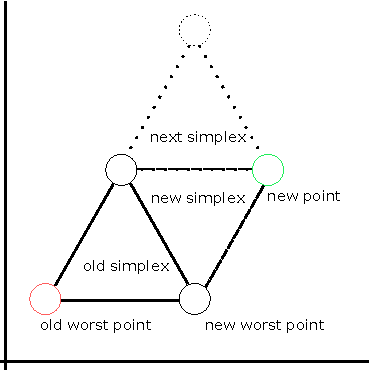
\includegraphics[width=0.4\textwidth]{Nelder-Mead}
\caption{Illustration of Nelder-Mead algorithm}\label{nelder-mead}
\end{figure}

Several derivative-free algorithms interpolate the objective-function with a simpler one. These methods starting with several evaluation points of the objective-function to build a simpler function on which it is possible to apply a known optimization method. Based on the result of the optimization, we can update the interpolation model and reiterate. Some possible interpolation methods include various polynomial interpolation methods, kriging \emph{etc.}

\section{Global Method}

While local optimization methods aim only for an optimum into a limited part of the search space, global optimization methods aim for the globally best solution of the problem. Global optimization methods concentrate on providing strategies to explore the search space.

Depending on the nature of the problem, it may be impossible to guarantee that the best solution will be found by any means other than a complete exploration of the search space (which is in itself an impossible task in the context of continuous optimization).

For example, suppose the following problem:

Minimize $f(x) =$ $\begin{cases}
 		 					0& \text{if } x = 1 \times 10^{-9}\\
 		 					1& \text{otherwise}
 		 			\end{cases}$
 		 			
There is no efficient strategy to find the global optimum to such a problem (unless knowing the equations, a thus the solution, beforehand).

Consequently, obtaining the global optimum of an optimization problem with certainty will be possible or not depending on the properties of the problem.
As with local optimization methods, several kinds of approaches have been proposed to solve problems with different properties.

\subsection{Exact Methods}

These methods aims at providing a guarantee about the optimality of the solution. These methods cannot be used for every optimization problem, as they need to use some properties of the problem to prove that the solution is a global optimum.

For example, as we said before, if an optimization problem is convex then a local solution is also a global solution. Consequently, for convex problems local optimization methods can be used with the guarantee that the solution found will be the best one.

As with linear programming, a specific class of problems belongs to the field of \emph{Quadratic Programming} (QP), and its extension \emph{Quadratic Constrained Quadratic Programming} (QCQP). QP concerns (non-convex\footnote{if the problem is convex, then we can use simple convex optimization techniques}) problems where the objective-function is quadratic (that is, a polynomial of degree 2) and all the constraints are linear. QCQP, as its name implies, concerns quadratic objectives and constraints.

Several adaptations of the Simplex method (presented is \ref{linear_optim}) for QP have been proposed (see for example \cite{wolfe1959simplex, dantzig1998linear, van1964simplicial}).

It is also very common to use relaxation techniques (\emph{Reformulation-Linearizion Techniques} or \emph{Semidefinite Programming}) to approximate the quadratic problem with a linear one. A widespread technique is to use a Branch and Cut, starting by replacing each non-linear term of the problem by a (linear) variable (for example, the term $x_ix_j$ would be replaced by the variable $v_{ij}$). For each replacement, a new constraint is added to maintain consistency of the solution (in our example, the new constraint would be $v_{ij} = x_ix_j$). Then these new constraints are themselves replaced by linear approximations.
To see more details on the different relaxations strategies, refer to \cite{audet2000branch}.

\subsection{Heuristic Methods}

When exact methods are too costly or non-applicable, it is often sufficient to get a good-enough solution. To this end it is possible to use heuristics to shorten the search space and ensure we obtain a solution in a reasonable time.

For example, a simple strategy can be to run a local optimization technique several times with different initialization points, in order to increase the coverage of the search space.

Expanding on this strategy is the \emph{Tabu search} metaheuristic. The idea of Tabu Search is to execute the same algorithm several times. To avoid converging  toward the same point, the previous solutions are memorized and are not allowed to be revisited. Thus the method has less chances to be quickly trapped in local optima.
The tabu search can be extended with several levels of memory to influence the search toward the most interesting regions of the search space.

Another class of heuristics introduces randomization into the search process in order to obtain a good coverage of the search space. These strategies are said to be \emph{stochastic}.

A very simple example of stochastic method is the Monte-Carlo algorithm. We start by choosing a point at random. Then we iteratively draw new points around the old one until we cannot improve the solution. Then we start again from another random point of the search space and continue until we reach an arbitrary termination criterion.
This method is very easy to put in practice, but can be quite costly in number of evaluations.

Another well-known technique is Simulated Annealing. This method is inspired from the annealing technique in metallurgy used to control the heating and cooling of a material in order to increase its properties.
Simulated annealing associate a global temperature and an energy measure to the state of the system (which represent the objective-function). Consequently the goal of the system is to minimize its energy. At each step, the method considers moving to one of the neighbors of the current point. The higher the temperature of the system, the more the system is susceptible to move, even if the neighbor is worse than the current point. As the temperature decreases, the system will favor more and more consistently solutions that decrease its energy.
The temperature of the system is reduced over time following a specific cooling schedule. For example the temperature could be decreased a each step, or could be reduced only when the system reached an equilibrium.

Some others stochastic techniques which can be applied, but are not restricted to, this kind of optimization problem are population-based algorithms, which will be presented in section \ref{population_based}.

\section{Conclusion on Continuous Optimization}

This overview of continuous optimization illustrates how the different optimization techniques range from very efficient but highly specialized methods to broad scope methods with slower and more costly strategies.
We have seen how the intuition provided by the NFL theorems is illustrated by the progression of the optimization techniques in general applicability and complexity.

An interesting observation is how specialized methods can concentrate on exploitation of the solutions, while generic methods are concerned with exploration of the search space. Indeed, the more we know about the structure of the problem, the easier it is to select a new search point. When lacking knowledge about the topology of the system, we need to be more concerned about exploring the search space.

From this basic compromise we can see how continuous optimization has given birth to such a plethora of methods, as every optimization technique is torn between this basic compromise.

All the methods we presented in this chapter share an inherent limitation due to the way they handle the problem. By using a centralized algorithm with a global view of the problem, in charge of the evaluating each point and deciding which new point to explore, these approaches require a complete re-evaluation of the entire problem at every iteration. In the next parts we will see increasingly complex problems, where the size of the problem, its topology and additional concerns not strictly related to the pure optimization make a complete evaluation of the problem increasingly costly, up to a point where applying methods such as the one we have presented in this chapter becomes too prohibitive.

\chapter{Multi-Objective Optimization}

Multi-Objective Optimization (MOO), also called multi-criteria optimization, departs significantly from previous categories of optimization in the fact that you have to consider multiple objective functions instead of only one. A main aspect of MOO is the way to conciliate these objectives, which are usually contradictory.
An example of real-world everyday MOO problem could be choosing the mean of transportation for a travel, trying to find a balance between speed and cost. Airplane is the fastest way of transportation, but is expensive. While car is slower, it is cheaper (if several people share the car). Train is slower than plane, more expensive than car, but can preferred as the best compromise. However, some solutions are strictly worse than others (in our example, renting an helicopter would probably be both more expensive and slower than buying a seat on a commercial airplane).
From this example we can see that, for an MOO problem, there rarely is a clear-cut \enquote{best} solution. And more importantly that even some solutions which are not optimum for \emph{any} of the objectives can be deemed satisfying. Only when each objective is completely independent, or when no objective is contradictory to another, then an MOO problem can be handled as a set of separated mono-objective optimization problems.
A solution vector which would be optimum for each objective is sometimes called \emph{utopia point}, or \emph{shadow minimum}, and is used as a reference comparison in some of the MOO techniques we present.

The formulation of a MOO problem does not differ significantly from the formulation of a \enquote{classical} optimization problem, the only difference being that instead of minimizing one objective function, we aim to minimize several ones:

\begin{align*}
\text{minimize } & (f_1(x), f_2(x), ..., f_n(x))\\
\text{subject to } & (x \in S)
\end{align*}

MOO problems are quite a radical departure from previous optimization problems type we have seen. Many approaches have been proposed, the majority of which can be separated in two categories: \emph{a priori} and \emph{a posteriori} approaches. \textbf{A priori approaches} aim at discriminating between the objectives \emph{before} the optimization process. This often consists into combining the different objectives into one, before applying a classical optimization method on the new, aggregated objective.
On the opposite, \textbf{a posteriori methods} try to provide a set of efficient solutions among which the decider will choose.
A priori approaches are considered easier, but not very efficient, whereas a posteriori approaches provide more diversity of solutions as well as more insight about the nature of the problem.
A third category can also be considered: the \emph{interactive} methods. Basically, these methods iterate between decision and search phases. For example, an interactive  method could work by quickly providing intermediate solutions to the decision-maker, which would in return refines the search using them.

We will now see some of the strategies have been proposed to deal with such problems. A recommended reading for the interested reader is the very complete overview by Marler \emph{et al.} in \cite{marler2004survey}. 

\section{A Priori Methods}

[[Utiliser un exemple simple pour comparaison]]

[[petite intro]]

\subsection{Objectives Aggregation}

The first approach is to transform the MOO problem back to a mono-objective optimization problem, by aggregating the different objectives into one. This can be expressed as follow : \(f_g = aggr(f_1, f_2, ..., f_n)\), where \(f_1, f_2, ..., f_n\) are the original objectives and \(f_g\) the aggregated one, which will be used with classical mono-objective optimization methods.

Concerning the choice of the aggregation function, different strategies can be used. The simplest strategy is to use a classical function such as addition, multiplication, mean, max or min of the objectives, and variations of the preceding (exponential sum, ...): these methods present the major drawback of requiring the aggregated values to be comparable. Going back to our travel example, is it relevant to simply add duration and cost ?

A slightly more sophisticated way is the weighted sum method, where a coefficient is attributed to each objective before adding them \cite{Marler2010} :

\[ f(x) =\displaystyle\sum_{i=1}^n w_i f_i(x) \]

Where $w_i$ are the coefficients representing the relative preferences between the objectives.

This method enables to express a preference between different objectives, as well as bringing back on comparable scale different objectives. However, one now has to decide of the coefficients to choose. Furthermore, this method can hide some information concerning the solution, for example an extremely poor result in one of the objectives, compensated by small improvements in all the others.  The method also present some limitations in the fact that it does not guarantee that the final solution will be an acceptable point, nor that a continuous variations of the points will leads to a continuous distribution of the solutions. it is also not possible to obtain solution points situated in a non convex region of the solution set \cite{marler2004survey}.

\subsection{Lexicographic Method}

In this iterative method, the objectives functions are arranged and optimized by order of importance. The result of the optimization at a given step becomes a constraint to satisfy for the following steps.

Formally, the problem becomes an ordered set of optimization problems, where each iteration can be expressed as follow:

\begin{align*}
\text{min } &f_i(x) \\
\text{subject to } &f_j(x) \leq f_j(x_j^*) \\
j = &1, ..., i-1
\end{align*}

It is also possible to replace inequalities by equality constraints \cite{stadler1988multicriteria}. Another variation, sometimes called hierarchical method \cite{osyczka1984multicriterion}, introduces a constraint relaxation coefficient $\delta$ where the new formulation of the constraints becomes:

\[ f_j(x) \leq \left(1 + \frac{\delta_j}{100}\right) f_j(x_j^*) \]

\subsection{$\epsilon$-constraint Method}

The $\epsilon$-constraint method \cite{4308298} proposes to change the expression of the problem by keeping only one objective (the one deemed the most important) and transforming the others into inequality constraints.

For example, the problem \[\text{min } f_1, f_2, ...,f_n\] where $f_1$ is deemed the most important objective would be transformed in
\begin{align*}
\text{min } &f_1 \\
\text{subject to } &f_2 \leq \epsilon_2, ..., f_n \leq \epsilon_n
\end{align*}

Where $\epsilon_2, ..., \epsilon_n$ must be chosen by the designer.
Depending of the selection of $\epsilon_2, ..., \epsilon_n$, it is possible to obtain a formulation where no feasible solution exists.
See \cite{marler2004survey} for a discussion about the different proposed methods for selecting $\epsilon$.

\subsection{Goal Programming}

The idea of Goal Programming (also called Target Vector Optimization) \cite{charnes1957management} is to fix for each objective an associated goal to reach. Each objective can be over- or underachieving its goal, allowing the designer to provide a rough idea of the initial design goals.

The new objective is to minimize the total deviation $\displaystyle\sum_{i=1}^n |f_i - g_i|$ where $g_i$ is the goal associated to objective $f_i$.

Goal Programming is very easy to use and quite popular, and can work even when the designer provided some unreachable goals, but provides no guarantee for the optimality of the solution.

\subsection{MinMax Method}

This method uses the separately attainable minima of the objectives (the so-called \emph{utopia point}) and try to minimize the maximum deviation of the objectives relative to those minima \cite{osyczka1984multicriterion}:

\[ \text{min } f = \text{ max } \left( \frac{f_i - f_i^0}{f_i^0} \right) \]

where $f_i^0$ represents the separately attainable minimum of the objective $f_i$.

This method can also be used similarly to Goal Programming, where the separately attainable minima are replaced by goal given by the designer.

A variant of this method, called weighted min-max, or weighted Tchebycheff method, uses the following formulation:

\[ \text{min } f = \text{ max } w_i |f_i - f_i^0| \]

where $w_i$ are coefficient provided by the designer.

\subsection{Analysis of a priori methods}

A priori methods provide a simple and efficient way to tackle the problem of multiple objectives, as they allow to reduce the problem to a mono-objective one.
However, a drawback of these methods is the need for the designer to have a good knowledge of the problem, to know the correct way to combine/compare the different objectives functions. In the general case, the designer may not have enough experience or information to make such decisions.

In the case where the designer would have enough knowledge to meaningfully use such a method, the introduction of this knowledge can risk to introduce a bias in the resulting solution, orienting the optimization process toward \enquote{standard} solutions at the expense of possible non-conventional ones.

Moreover, aggregation techniques tend to break when the objectives are not comparable, requiring once more knowledge from the designer to introduce adjustment coefficients to re-equilibrate the aggregation function.

\section{A Posteriori Methods}

We have seen that, while convenient, \emph{a priori} methods can be quite restrictive. By choosing beforehand a way to aggregate the different objectives, we lose in diversity of solutions and influence the result of the optimization process.

\subsection{Pareto Dominance}

A radically different approach has been proposed, using the concepts of Pareto dominance and Pareto optimality. These concepts were originally developed in economical sciences first by Francis Edgeworth and later Vilfredo Pareto \cite{nla.cat-vn2742363}. The initial application of the concepts was to propose a minimal definition of \enquote{efficiency}, regarding allocation of resources inside an economical system.

The main idea is that a state where it is impossible to improve the resources allocation for an individual without worsening the situation of at least another is described as \emph{Pareto efficient}, or \emph{Pareto optimal}.

Conversely, if from a system state A it is possible to find a new state B where at least one individual's situation is improved without worsening the situation of another, the state A will be said to be \emph{Pareto inefficient}. The state B will be said to \emph{dominate} the state A in terms of Pareto optimality, and the passage from A to B will said to be a \emph{Pareto improvement}. This relation of Pareto dominance is usually noted \(\prec\).

\definition{Pareto-dominance}{Given A and B two vectors describing different resources allocations in a system, \(A \prec B \Leftrightarrow (\forall i \text{ }A_i \leq B_i \land \exists j \text{ } A_j < B_j\)). }

Note that, to complicate a little the understanding of this notion, the definition of domination depends of whether we actually want to \emph{maximize} or \emph{minimize} the resource allocation. Note that in this definition we wanted to maximize resources allocation, so \(A \prec B\) reads \enquote{B dominates A}. If we want to \emph{minimize} the allocation, the meaning is inverted and  \(A \prec B\) reads \enquote{A dominates B}.
As it is the standard convention in optimization to express problems in terms of minimization, for the rest of this thesis we will use \(A \prec B\) with the meaning of \enquote{A dominates B}, unless otherwise specified.

Based on this relation of dominance, it is possible to provide a definition of Pareto-optimality.

\definition{Pareto-optimality}{A solution vector that is not dominated by any other possible solution is said to be Pareto-optimal.}

\definition{Pareto front}{the set of Pareto-optimal solutions.}

It is also possible to classify the solutions by rank: a solution which is dominated by no other is said to be of rank 0 (and to be Pareto-optimal). A solution which is dominated by at most a solution of rank 0 is said to be of rank 1 and so on.

As a remark, these definitions of efficiency and optimality do not give any information about the fairness of the allocation, or the well-being of the involved parties. From this point of view, a monopolistic situation where one individual would control all the available resources is as optimal as a situation where all the resources are equally divided between the individuals.

These definitions of dominance and optimality can be used to characterize the possible solutions of MOO problem. In this case, the problem is not to find an optimal solution anymore, but to find the Pareto front of the problem.

An illustration of a Pareto front can be seen on figure \ref{Front_Pareto}. The elements A and B are Pareto-optimal, while C is not.

\begin{figure}
\centering
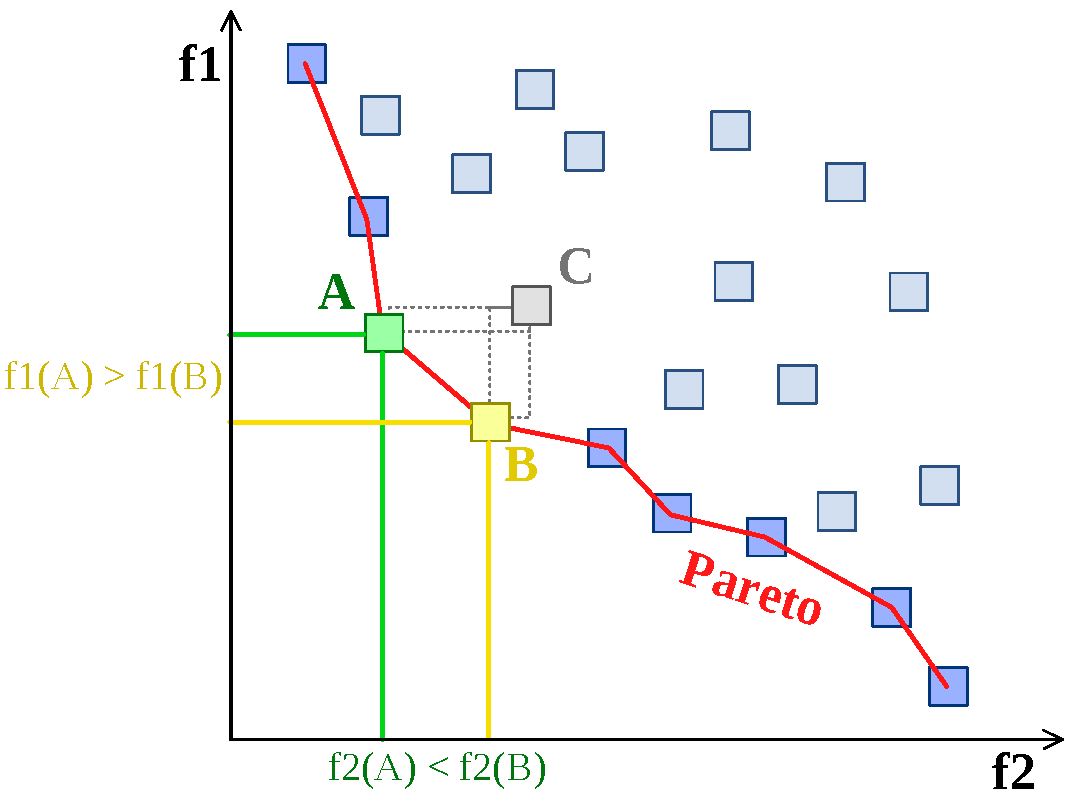
\includegraphics[width=0.4\paperwidth]{Front_pareto}\\
%\hfill\includegraphics[width=6em]{by-sa} \href{http://en.wikipedia.org/wiki/File:Front_pareto.svg}{\begin{small}Johann Dréo\end{small}}
\caption{Illustration of the notion of Pareto Front (CC-BY-SA \href{http://en.wikipedia.org/wiki/File:Front_pareto.svg}{Johann Dréo})}

\label{Front_Pareto}
\end{figure}

\subsection{Evolutionary Algorithms}

[[Talk about scalability problems -> "Techniques for Highly Multiobjective Optimisation: Some Nondominated Points are Better than Others" by David Corne and Joshua Knowles]]

A widespread strategy to find the Pareto front is to use [[population-based]] metaheuristics, such as Multi-Objective Evolutionary Algorithms (MOEA). 

Historically, evolutionary algorithms are divided in two main categories, based on whether or not they use elitism mechanisms, with some consensus concerning the superiority of elitist algorithms.

\subsubsection{Non-elitist evolutionary algorithms}

These \enquote{first-generation} algorithms 
[[Vector Evaluated Genetic Algorithm (VEGA) Schaffer (1985) => Non Pareto]

[[  Goldberg and Richardson (1987) =>  Simple Pareto domination scheme. • Sharing on whole population]]


\subsubsection{Elitist evolutionary algorithms}

Non-elitist techniques often have trouble to converge toward the Patero front, as well as to keep a good optimum diversity and to spread on the front. To remedy that issue, elitist algorithms propose various additional mechanisms:
\begin{compactitem}
\item maintaining an external \enquote{archive} population containing the optimum found so far
\item using clustering technique to spread the solutions among the Pareto front
\item introducing an additional preferential bias for non-dominated solution

[[Signal that evolutionary algorithms have difficulties with more than two objectives ?]]

\subsubsection{Analysis of evolutionary algorithms}

Evolutionary algorithms propose an interesting Nature-inspired mechanism for solving MOO problems. By maintaining a population of candidate solutions and using selection pressure mechanisms, they make possible a throughout exploration of the Pareto front. The compromise between exploration and exploitation will be determined by the parametrization of the different genetic operators and the selection/crossing process. While this aspect can prove to be advantageous for the potential flexibility it brings, it is often difficult to guess what are the relevant parameters values. Consequently it can be necessary to iterate the optimization process in order to manually fine-tune the parameters.

A major limitation of these methods is their potential computational cost. Such algorithms need to evaluate a relatively large number of candidate in order to create a good population of solutions. Computing all the candidate solutions can be prohibitive for computationally expensive problems.

It has also be noted in [[Techniques for highly multiobjective optimisation: some nondominated points are better than others]] that many MOEA have poor scalability performances in regard of the number of objectives. This degradation of performances is attributed to the combined factors of:
\begin{compactitem}
\item the exponential complexity increase of the procedures in regard of the number of objectives
\item the increase of non-dominated solution caused by the additional objectives
\item the limited size of the archived population in regard to the number of potential candidates
\end{compactitem}

\chapter{Advanced Concepts for Optimization}

In this chapter, we present two advanced concepts regarding optimization: optimization under uncertainties and optimization in dynamic environments. In both cases, the goal is no longer to only find the best solution to the optimization problem, as the context of this problem implies some specific requirements.

In optimization under uncertainties, we take into account the fact that we are not in a ideal mathematical world: the instantiation of the problem in the physical world presents some limitations (for instance the length of a manufactured object is often not exactly as expected) and our knowledge (of a model, a process, etc.) is pervaded with imprecision.

For optimization in dynamic environments, the objective functions are deterministic but change over time (and so do the optima). This kind of problem requires specific optimization techniques able to adapt to this changing goal.

\section{Optimization Under Uncertainties}\label{SOA_uncertainties}

In a pure mathematical world, all models are perfectly correct and have an infinite precision. However, in the physical world, our knowledge can be extremely limited. Moreover, high precision models can require a long time to be computed, making them prohibitively costly when used in the context of an optimization process. Finally, when the optimization problem is complex, a small approximation can result in large variations of the output, if the system is sensitive to parameters variations.

In order to tackle these issues, several works have been done to take into account uncertainties into the optimization process. We propose to make a quick tour of the different ways which have been proposed to model and propagate uncertainties.
A major concern regarding the modeling of uncertainties is the uncertainties \emph{propagation}. 

\subsection{Several types of uncertainties}

A distinction is usually made between \emph{aleatory} uncertainties and \emph{epistemic} uncertainties.

\textbf{Aleatory uncertainties} are inherent to the studied system. They can represent for example variability in the material used, a physical variation regarding the manufacturing of some piece, the meteorological conditions to which a device will be exposed etc.
These uncertainties are \emph{irreducible} as it is impossible to remove them with a better analysis of the system.

\textbf{Epistemic uncertainties} result from an incomplete knowledge regarding the system. These uncertainties can result from a limited set of data or lack of knowledge regarding a physical phenomenon.
The uncertainties are \emph{reducible} as it is possible to remove them with a better analysis of the system. However, removing epistemic uncertainty can often be too costly or too difficult in practice, thus they still need to be taken into account during the optimization process.

For example, let's suppose we work on a model taking two variables as input and producing an output: $z=f(x,y)$.
Based on known uncertainties on the inputs and the model, how easy is it to combine and propagate these information to determine the uncertainty regarding the output ? Or more formally, can we provide a propagator $P$ such as $u_z = P(u_x, u_y, u_f)$ (where $u_i$ is the uncertainty associated with the element $i$)? As we will see, the ease to obtain such a propagator $P$ depends on the chosen way to model the uncertainties.

\subsection{Uncertainties Modeling Techniques}

[[small intro]]

\subsubsection{Probability Theory}

Using the probability theory, uncertainty can be modeled using a distribution function. This modeling provides the advantages of a well-studied theoretical foundation, providing well-known combination and propagation techniques.

Aleatory uncertainties can be characterized by obtaining a distribution function from a data sample.
Well-known statistical techniques can be used to see for example if a data sample follows a known probability distribution, measuring \emph{goodness of fit}, that is, how well a data sample follows a given model, such as the Kolmogorov-Smirnov test \cite{Massey_1951}. 
However, care must be taken as these techniques can introduce some more epistemic uncertainties which can lead to misleading results (for example in the case of insufficient data samples).

Concerning epistemic uncertainty, it can be more difficult to estimate a relevant distribution function  [[TO EXPAND]]

\subsubsection{Interval Analysis}

Interval analysis can be an alternative to probability theory when the lack of information impedes modeling with a probability distribution, but where the uncertainty can still be bounded within a certain domain.
How easy is it to propagate intervals depends on the involved models. For example in the case of a monotonic function the lower and upper bounds can be determined easily. In the general case, determining the boundaries is equivalent to solve an optimization problem and can thus be solved by using optimization algorithms. In the most extreme cases, one can apply sampling techniques, but this can become quite expensive.
For some examples of existing techniques, one can refer to \cite{Kreinovich_2008}.

A limit of interval analysis is the lack of a measure equivalent to probability, which limits the usefulness of this representation in the general case. This modeling can still prove useful in the context of worst case studies where inputs variables can be bounded with accuracy.

\subsubsection{Fuzzy Sets}

Fuzzy sets \cite{zadeh1965fuzzy} can be seen as a compromise for when we still lack enough information to use probability theory, but we have more knowledge than just the bounds of the uncertainty.

Basically, fuzzy sets are sets where the membership of an element to the set is not absolute but gradual.
In classical set theory, an element is or is not a member of a set. This notion can be formalized as a function $f_S: X \rightarrow \{0,1\}$ where 
$\left\{
 		 \begin{array}{rcr}
			f_S(x) = 0 \Leftrightarrow x \not\in S\\
			f_S(x) = 1 \Leftrightarrow x \in S
		\end{array}
	\right. $

In the context of fuzzy sets, the equivalent function can be formalized as $f_S: X \rightarrow [0, 1]$, where $f_S(x)$ represents the degree of membership of $x$ to $S$. A value of 1 indicates a total membership to S, a value of 0 a complete absence of membership to S and the values in between specific degrees of membership.
In this regard, fuzzy sets can be seen as a generalization of classical sets.

Fuzzy sets quantification capability to represent vague information makes it attractive to model epistemic uncertainty, as it is more precise than interval analysis and well-suited to express expert knowledge. However this modeling is less powerful and expressive than probability theory, lacking for example a mean to represent an uncertainty measure equivalent to the probability of the probability theory. Indeed, the membership function is insufficient to characterize the likelihood of non-connected events.
To overcome this limitation, the fuzzy set theory was extended into the possibility theory.

\subsubsection{Possibility Theory}

Possibility theory \cite{zadeh1978fuzzy} seems similar to probability theory. However, they are based on axioms which diverge on a fundamental point.
The probability theory is based on the axiom of \emph{additivity}, which says that for two disjoints sets $U$ and $V$, $P(U \cup V) = P(U)+ P(V)$, that is the probability of at least one of two mutually exclusive events to be verified is the sum of the probabilities of each event.

The possibility theory contains instead an axiom of \emph{sub-additivity} saying that for two disjoints sets $U$ and $V$, $\Pi(U \cup V) = \text{max }(\Pi(U), \Pi(V))$ (where $\Pi(X)$ reads as \enquote{possibility of X}).

Let's take the basic example of a door which can be either open or closed. If we assume \enquote{the door is closed} has a probability of 1, it must follow that \enquote{the door is open} has a probability of 0, since the sum of these two complementary events must be 1.

In the context of possibility theory, if we state that the possibility of \enquote{the door is closed} is 1, it is not incompatible with the possibility of the door to be open to be, for example, 0.4.

The intuition behind this difference is that probability theory applies to the reality, while possibility theory applies to the knowledge one has regarding the reality, taking into account the \enquote{fuzziness} of one's knowledge. To cite the definition proposed by Nikolaidis et al. \cite{nikolaidis:386}:
\begin{quote}
\enquote{Possibility measures the degree to which: a) A person considers that an event can
occur, or b) The degree to which the available evidence does not contradict the
hypothesis that the event can occur.}
\end{quote}

As well as the notion of \emph{possibility}, possibility theory introduces the notion of \emph{necessity}. Basically, $Nec(U) = 1 - \Pi(\bar{U})$.
This definition implies several interesting properties:

$\left\{
\begin{array}{l}
Nec(U) \leq \Pi(U)\\
Nec(U) + \Pi(\bar{U}) = 1\\
\text{either } \Pi(U) = 1 \text{ or } Nec(U) = 0\\
\end{array}
\right.$

Necessity and possibility of an event $e$ can be viewed as lower and upper bounds to the probability of $e$.

Possibility theory offers numerous tools similar to the ones of probability theory (so much that it was debated if the two theories are really different or if possibility theory was just a variation on probability theory). However, the capability of this theory to model expert knowledge specifically has made it quite popular in the context of uncertainty modeling.

\subsubsection{Evidence Theory}

Evidence theory \cite{shafer1976mathematical}, also known as Dempster-Shafer theory (DST), takes into account available evidences to provide a degree of belief concerning a fact.
The basic idea of this theory is to represent the notion that the more evidences seem to confirm a proposition, the more we can believe the proposition to be true.

Evidence theory represents a proposition as a set of elements. Thus some propositions can include others propositions (following the basic set inclusion definition). To these sets are assigned a basic belief assignment (BBA), also called \emph{mass}.

From this mass can be calculated two measures:

\begin{itemize}
\item \emph{Belief:} $bel(S) = \displaystyle\sum_{S'\subseteq{S}} mass(S')$
\item \emph{Plausibility:} $pl(S) = \displaystyle\sum_{S'|S' \cap S \neq \emptyset} mass(S')$
\end{itemize}

The mass measurement represents the amount of evidences which support the proposition, the likelihood of $S$. The belief and plausibility can be seen as lower and upper bounds to this likelihood.

Once again we can obtain some interesting properties regarding these measures:

$\left\{
\begin{array}{l}
bel(S) \leq mass(S) \leq pl(S)\\
pl(S) = 1 - bel(\bar{S})\\
bl(S) + bl(\bar{s}) \leq 1\\
pl(S) + pl(\bar{s}) \geq 1\\
\end{array}
\right.$

As with possibility theory, belief and plausibility can be used as lower and upper bounds for probability.

Several rules have been proposed to combine informations coming from different (potentially conflicting) sources. To see an overview of these proposals, the reader can refer to \cite{sentz2002combination}.

\subsubsection{Analysis of uncertainties modeling}

[[NEED AN ANALYSIS OF UNCERTAINTY MODELING]]

\subsection{Using Uncertainty for Robust Optimization}

[[From Jpg : un schéma exemple aussi avec un optimum global fragile et un optimum local robuste poru marquer l'idée en un coup d'oeil.]]

\subsubsection{Taguchi Method - The firsts steps of Robust Optimization }

Robust optimization tries to provide a solution which is both good and insensible to small variations of the inputs.

The research on robust optimization has been initiated with Taguchi's robust design methodology\cite{tsui1992overview}, aiming at improving the quality of manufactured goods.
In his methodology, Taguchi proposes a three-stages process :
\begin{itemize}
\item System design, where the designers determine the overall structure of the product at a high conceptual level;
\item Parameter design, where the optimal values of the design variables are determined;
\item Tolerance design, which focuses on reducing the variability of the  various parameters to fix an acceptable limit to the variability of quality for the product.
\end{itemize}

To help the designers during the parameter design phase, Taguchi introduced several measures, among them the Signal-to-Noise (SN) ratios. These ratios are used to estimate the sensitivity of a performance of the product to variations. Each ratio relates to a possible goal regarding the studied performance: larger the better, smaller the better, on target the best. These ratios are respectively noted $SN_L$, $SN_S$ and $SN_T$.
By simulation or experimentation, one must first produce a data set.

The $SN_L$ and $SN_S$ can be directly calculated as

\[SN_L = -10\text{log}\left( \frac{1}{n} \sum_{i=1}^n \frac{1}{y_i^2} \right)\]
\[SN_S = -10\text{log}\left( \frac{1}{n} \sum_{i=1}^n y_i^2 \right)\]

For $SN_T$, we need first to measure the mean response, given by $\bar{y} = \frac{1}{n}\displaystyle\sum_{i=1}^n y_i$
This mean can then be used to calculate the standard deviation as follows 
\[S = \sqrt{\sum_{i=1}^n \frac{(y_i - \bar{y})^2}{n-1}}\]

 $SN_T$ can then be calculated as
 
 \[ SN_T = 10\text{log}\left(\frac{\bar{y}^2}{S^2}\right) \]
 
To reduce the sensitivity of the solution to noise, the SN ratio must be maximized. To this end, Taguchi use the Design of Experiment\cite{sacks1989design}, a statistical procedure for determining the effect of multiple inputs on a desired output. by evaluation different designs using different noise factors (temperature, pressure \emph{etc.}), it is possible to obtain an array of SN rations on which a statistical data analysis allows to identify which design provides the best performances.

Tagushi was the first to propose a way to take in account the uncertainties in design. As it is nearly inevitable for such pioneering work, his approach suffers from several limitations. As the number of parameters increases, so do the number of experiments (for $N$ parameters and $M$ noise factors we need $2^N$ designs and $M2^N$ experiments). Moreover, the statistical measures proposed by Tagushi has been subject to much debate (for a discussion of these measures see \cite{nair1992taguchi}). However, Tagushi opened the way for the other methods in the field.

\section{Optimization in Dynamic Environments with Population-Based Algorithms}\label{population_based}

A special case of optimization is optimization in dynamic environments. In this kind of problem, the objective-function is likely to change with time. To avoid confusion, optimization in dynamic environment is distinct from \emph{dynamic programming} (another optimization field not addressed here) in the fact that the changes of the objective-function \emph{are not known beforehand}. Thus it is not possible to anticipate these changes during solving.
Classical optimization techniques fail to solve this kind of problem as they are not meant to take into account these dynamics. These problems require specific optimization techniques, able to both find a moving optimum and to follow it when it changes.

The main field concerning solving optimization problems in dynamic environment is population-based optimization (also called \emph{evolutionary computation}). Population-based optimization is a very prolific and diversified field, whose algorithms are often inspired from the observation of natural populations behavior. The underlying principle of this kind of algorithm is the use of a population of entities which are spread within the search space, with specific strategies in order to iteratively progress toward the solution. These strategies involve transformations applied to the entities that compose the population (moving, creating or destroying or otherwise altering them).

\subsection{Evolutionary Algorithms}

Evolutionary Algorithms (EA) are based on a Darwinist selection process. The main idea is to maintain a population of solutions which is iteratively improved by selecting, crossing and mutating the best individuals in regard of a given \emph{fitness function}. Most EA are based on the algorithm shown in algorithm \ref{evo_algo}.

\begin{algorithm}
\caption{Evolutionary Algorithm Pseudocode}
\label{evo_algo}

	generate initial population\;
	evaluate fitness of individuals\;
	\Repeat{termination condition reached}{
		evaluate select best-fit individuals\;
		produce offspring based on selected individuals\;
		evaluate fitness of offspring\;
		replace least-fit population with offspring\;
	}	
\end{algorithm}

\emph{Genetic algorithms} \cite{holland1992adaptation}, by far the most often used type of EA in optimization. In the context of genetic algorithms, each individual entity is defined by a specific \emph{genotype}, which represent a possible solution to the problem.
Like we said previously, a global \emph{fitness function} is defined, which is used to evaluate the solutions represented by these individuals.

Regarding a continuous optimization problem, the genotype of an entity would be a set of values assigned to the inputs of the problem, while the fitness function would be the objective-function.

The optimization process iterates over two phases: \emph{selection} and \emph{generation of a new population}.
In the selection phase, a subset of the current population is selected to be used in the generation of the new population. In the most basic approach, the selected individuals are the ones which obtain the best scores on the fitness function.
The second phase generates a new population, based on the selected individuals. To produce the new population, a set of biology-inspired genetic operators is used. Two of the most common genetic operators are \emph{crossover} and \emph{mutation}. The crossover is the creation of a new individual, whose genotype is based on the combination  of two randomly selected \enquote{parents}. The mutation consists in randomly changing a part of the genotype of an individual.

Together, these two operators can be seen as representatives of the exploitation versus exploration dilemma. The crossover operation is an attempt to exploit the best solutions found so far, while the mutation is done to maintain diversity in the population. 

Most genetic algorithms proposals work on variations on these two phases. For example, some techniques will select not only the best fitted individuals, but also a small part of low fitted ones in order to increase the exploration of the search space. Some variants also modify the genetic operators or introduce additional ones. For example it is possible to do the crossover using more than two parents, or to introduce the notions of groups and migration.

\subsection{Swarm Algorithms}

Swarm algorithms focus on the decentralized exploration of the search space by a population of entities (commonly called \emph{agents} or \emph{boids}). These entities usually have only a local perception of the search space and individually decide how to move using simple rules.

Particle Swarm Optimization (PSO) \cite{kennedy1995particle} is inspired from the flocking behavior of social animals (such as birds, fishes or bees). PSO consists of a swarm of particles initially spread across the search space. Each particle $i$ can perceive its neighborhood and moves according to its current position $x_i$ and velocity vector $\overrightarrow{v_i}$.
During solving, each particle memorizes the best solution it found so far $x_i^*$. Based this information, a global best $x_g^*$ is calculated and provided to each particle for the next iteration.
At each step, a particle updates its velocity based on the current velocity, its local best value and the global best value found. Then it moves according to its current position and velocity. The influence of these various parameters can be modulated using the coefficients $w$, representing the inertia, $c_l$ representing the influence of the local best solution and $c_g$, representing the influence of the global best solution.

Algorithm \ref{PSO_algo} shows the principle of PSO.

\begin{algorithm}
\caption{PSO iteration}\label{PSO_algo}

	\ForEach{particle}{
		$\overrightarrow{v_i}(t) = w.\overrightarrow{v_i}(t-1) + c_l.rnd(x_i^*(t-1)-x_i(t-1)) + c_g.rnd(x_g^*(t-1)-x_i(t-1))$\;
		$x_i(t) = x_i(t-1)+\overrightarrow{v_i}(t)$\;
		\If{$x_i(t)$ better than $x_i^*$}{
			$x_i^*$ = $x_i(t)$\;
		}
	}
	$x_g^*$ = best of $x_i^*, \forall i$\;

\end{algorithm}

\subsection{Analysis of Population-Based Algorithms}

Population-based algorithms tackle the problem of a dynamic environment by maintaining a diverse population of solutions. Of course this kind of algorithm does not avoid the dilemma of exploration versus exploitation, having to choose between maintaining a high diversity of solutions and concentrating the population around the most promising regions. Most of these techniques includes specific parameters to adjust the solving process toward more exploration or more exploitation (for example the coefficients regarding current velocity, local and global optima in PSO). The choice of finding the best parameters is once again handed down to the person which applies the method.

Another inconvenient of Population-based approaches is the high number of evaluations they need to make. Indeed, each individual will require at least one evaluation of the whole problem. If the problem is very costly to evaluate, this kind of method may not be worth considering.

Finally, this kind of method often has some difficulties to scale with the complexity of the problem. Genetic algorithms will often have difficulties solving problems where the search space is very large, and swarm algorithms will present difficulties when the 
search space has a high number of dimensions or with chaotic topologies.

\section{Conclusion on Advanced Concepts for Optimization}

After studying the needs for taking in account multiple objectives, we have seen in this chapter how optimization problems often need integrate more advanced concerns than solely finding the best solution to a problem. With MOO, we had seen that the \enquote{best solution} was often a compromise between multiple objectives. We have now seen in this chapter that the best solution can sometimes be a solution which is suboptimal, but more robust than the analytical optimum, or that the best solution could change with the time.

The analytical methods we have studied at the beginning of this part are quite inadequate to take in account these additional concerns, which are part of the real-world concerns faced by the designers and engineers. For this reason, new methods have been developed to get around these limitation. In both robust optimization and optimization in a dynamic environment, these methods usually work by making a large number of evaluations, either to study the robustness of a solution or to maintain a population of representative solutions.

We will see in the next chapter how these methods are still insufficient to handle the most complex continuous optimization problems, due to the very fundamental assumption they make by considering the objective-function(s) to be trivial to evaluate. We will now see a kind of optimization problems which are so complex that a single evaluation of the problem is considered a cost, and some methods which have been proposed to handle such problems.

\chapter{Multidisciplinary Optimization}\label{MDO_chapter}

Multidisciplinary Design Optimization (MDO), often abbreviated Multidisciplinary Optimization , concerns the optimization of complex systems which involves several interacting disciplines. Each discipline in itself can contain this own variables, objectives and constraints. These problems often involve several of the optimization problematics we examined in the previous chapters (non-linearity, multiples objectives and constraints, uncertainties etc.) and are usually too complex to be handled by classical optimization methods for several reasons. Evaluating the global function of the problem is considered to be expensive, as it involve complicated models, requiring extensive calculus. The optimization problem usually contains not just contradictory objectives, but whole conflicting disciplines. The complexity of the problem is also increased by the fact that the different parts of the problem are interdependent and can potentially add several layers of intermediate calculus, making difficult to estimate the impact of the different design variables on the different criteria.\\
In this regard, we can say that MDO problems tend to regroup and amplify all the difficulties encountered with the previous types of optimization problems.

These kinds of problems are commonplace in the industry, especially in complex systems design such as aeronautic and aerospace engineering, where parts of the design are often done by different experts teams. For example designing an aircraft can be formalized as a MDO problem involving several disciplines such as mechanics, aerodynamics, acoustics etc. (see \figurename\ \ref{aero-disc}).

\begin{figure}
\centering
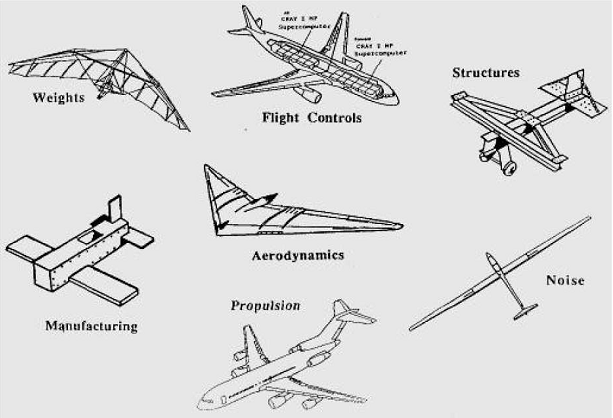
\includegraphics[width=0.4\paperwidth]{Disciplines_Avion}
\caption{Examples of aeronautics disciplines [[SOURCE]]}
\label{aero-disc}
\end{figure}

To handle such complex systems, most strategies propose to decompose it into several sub-systems of lesser complexity. Concerning engineering, several decomposition strategies have been proposed\cite{kusiak1995decomposition}:

\begin{itemize}
\item product (also called object) decomposition, based on the physical components of the system. This kind of decomposition is not always adequate and often subjective;
\item process  (also called sequential) decomposition, based on the workflow of elements/informations involved into the design process. This decomposition is most adequate when the design process is linear.
\item domain (also called aspect) decomposition, based on the knowledge domains, the disciplines, involved. This kind of decomposition is the basis of MDO methods.
\end{itemize}

The AIAA MDO Technical Committee proposed the following definition of MDO\footnote{\url{https://info.aiaa.org/tac/adsg/MDOTC/Web\%20Pages/aboutmdo.aspx}} \cite{american1991current}:
 \begin{quote}\textit{
\enquote{A methodology for the design of complex engineering systems and subsystems that coherently exploits the synergism of mutually interacting phenomena.}}
\end{quote}
MDO methods are not optimization methods \emph{per se}. Instead they focus on providing an optimization strategy for optimizing the different disciplines while maintaining a global coherence. In fact, the optimization of the disciplines is done using classical optimization methods such as presented above. In this regard, MDO methods could be seen as optimization meta-methods, or methodologies, as they provide methods to best apply optimization methods to a complex problem. Martin and Lambe \cite{Lambe:2011:A} note several other terms have been used in the literature: \enquote{architecture}, \enquote{method}, \enquote{methodology}, \enquote{problem formulation}, \enquote{strategy}, \enquote{procedure} or \enquote{algorithm}.

Alexandrov and Lewis illustrated their discussion on Collaborative Optimization \cite{NataliaM.:2000:ACA:886733} with the following theoretical test case:

\begin{align*}
a_1 &= A_1(s, l_1, a_2) \\
a_2 &= A_2(s, l_2, a_1) \\
\text{minimize } &f(s, a_1, a_2) \\
\text{subject to } &g1(s, l_1, a_1) \geq 0 \\
								&g2(s, l_2, a_2) \geq 0
\end{align*}

It can be noted that this formulation does not differ from the standard optimization problem formulation. Indeed, as noted by Martin and Lambe \cite{Lambe:2011:A}:
 \begin{quote}
 \textit{
 \enquote{If we ignore the discipline boundaries, an MDO problem is nothing more than a standard constrained nonlinear programming problem: we must find the values of the design variables that maximize or minimize a particular objective function, subject to the constraints.}}
\end{quote}
A very common strategy used by most MDO methods is to reformulate the problem to \emph{decouple} variables which are shared among the disciplines. 
For example, the following optimization problem:

\begin{align*}
\text{Minimize } f(f_1(x), f_2(x))
\end{align*}

(where $f_1$ and $f_2$ represent two disciplines depending on $x$)

could become :

\begin{align*}
\text{Minimize } &f(f_1(x_1), f_2(x_2))\\
\text{s.t. } &x_1=x_2
\end{align*}

The shared variable $x$ has been replaced by two independent variables $x_1$ and $x_2$, and a new constraint $x_1=x_2$ has been added to ensure the consistency of the design.

Several specific terms are in use in the domain of MDO:

\begin{itemize}

\item \emph{Design variable}: a variable of the problem which can be chosen by the designer. The goal of the optimization process is to find good values for the design variables of the problem. A design variable is said to be \emph{local} (or \emph{private}) if it is relevant to only one discipline, or \emph{shared} (or \emph{public}) if it is used by several of them.

\item \emph{Discipline Analysis}: The evaluation of the output variables of a single discipline, based on given values for the input variables, ensuring that all the values involved in the discipline are consistent.

\item \emph{Multidisciplinary Analysis (MDA)}: The evaluation of the complete problem based on given values for the input variables. In order to find a set of consistent values, the different disciplines may need to be evaluated several times.

\item \emph{Optimizer/Solver}: A classical optimization technique, such as the ones we have seen in the previous chapters. These optimizers can be applied to the problem as a whole or to specific parts.

\end{itemize}

The classical approach to categorize MDO methods was to separate mono- and multi-level methods.
Mono-level methods use a single optimizer and a non hierarchical structure, while multi-level methods use a hierarchical structure and possibly several optimizers.

%\section{An Illustration of Coupled Systems Problematics: Fixed Point Iteration}
%
%[[What tot do with this ??]]
%
%To illustrate the difficulties caused by coupled system, let's introduce the Fixed Point problem.
%
%\subsection{Fixed Point problem}
%
%Initially, the problematic of fixed point is the following:
%
%\begin{quote}\enquote{Considering a function $f(x)$, does a $x_{fp}$ exists for which $f(x_{fp}) = x_{fp}$?}\end{quote}
%
%If such $x_{fp}$ exists, then it is called a \emph{fixed point} of $f$
%
%\definition{fixed point}{$x_{fp}$ is a fixed point of $f \Leftrightarrow f(x_{fp}) = x_{fp}$}
%
%Not every function has a fixed point, and some functions can have more than one. For example the function
%
%$$f(x)=x+1$$
%
%has no fixed point (there is no $x$ for which $x = x+1$), while the function
%
%$$f(x) = x^3$$
%
%has three fixed points: -1, 0 and 1 (cf figure \ref{fixed_points_x_3}).
%
%\begin{figure}
%\centering
%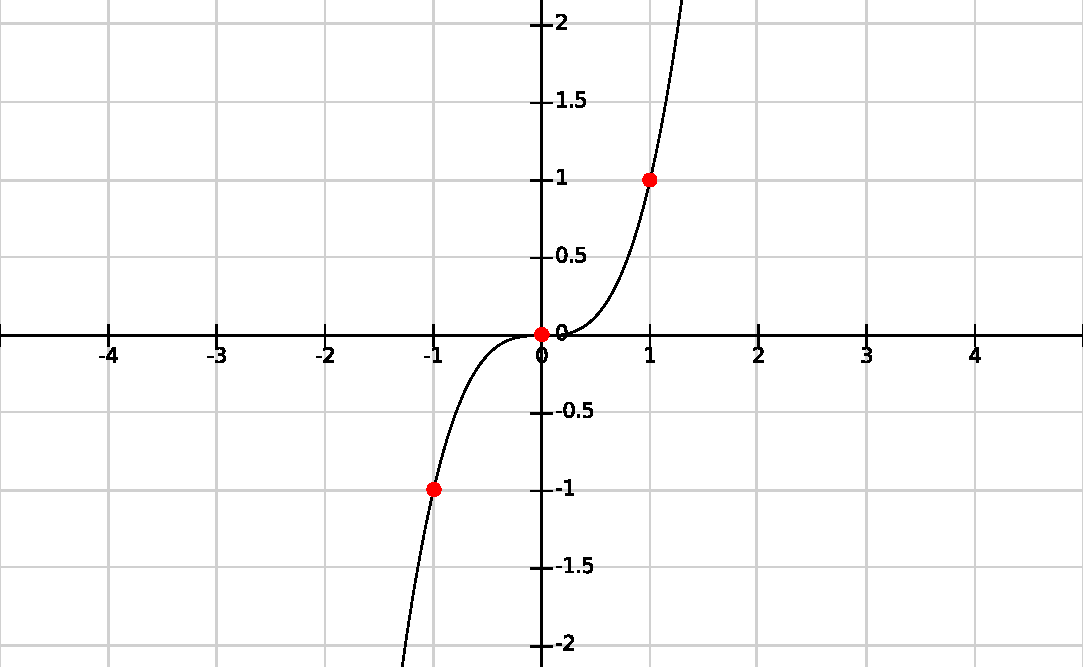
\includegraphics[width=0.4\paperwidth]{fixed_point_x_cube_withdots}
%\caption{$f(x)=x^{3}$ and its fixed points, (in dashed grey, the function $y = x$)}
%\label{fixed_points_x_3}
%\end{figure}
%
%An obvious property of fixed points is that $x_{fp} = f(x_{fp}) = f(f(x_{fp}))$ ...
%
%A fixed point can be \emph{attracting} or \emph{repelling}. A fixed point is said to be attracting when the system converges towards it when iterating over $f$ in its neighborhood. Conversely, a fixed point is repelling if we diverge while doing so. A fixed point which is neither attracting nor repelling is said to be \emph{neutral}.
%
%[[insert diagram of attractive and repelling fixed points]]
%
%A fixed point $x_{fp}$ will be attracting if $|f'(x_{fp}| < 0$.\\
%If $|f'(x_{fp}| > 0$ then the fixed point is repelling.\\
%Finally if $|f'(x_{fp}| = 0$ then $x_{fp}$ is neutral.
%
%
%\subsection{Fixed Point with Coupled Functions}
%
%The notion of fixed point can be extended to coupled functions. [[TODO?]]

\section{Mono-Level Methods}

\subsection{Multidisciplinary Feasible}

MultiDisciplinary Feasible (MDF) \cite{cramer1994problem}, represented in \figurename{} \ref{mdf_graph}, is the most basic and classical MDO method. This approach ensures at each optimization step that the design is consistent as a whole, taking into account all the disciplines together (hence the name). The optimizer only use the design variables, objective functions and constraints.
Basically, MDF alternates between a MDA (multidisciplinary analysis) and a global optimization phase, ensuring the design to be globally consistent at each optimization step. At each step, the result proposed by the optimizer is used to do a full MDF whose results are used in return for the next optimization iteration.

\begin{wrapfigure}{r}{0.5\textwidth}
\centering
\includegraphics[width=0.4\textwidth]{mdo_mdf}
\caption{MDF method}\label{mdf_graph}
\end{wrapfigure}

As it is so straightforward, MDF requires no reformulation of the problem, unlike most of the others MDO methods, and in so is really easy to use. As the design is consistent at each step, the optimization process can provide a solution at any time (but it will not guarantee that the proposed solution will satisfy the constraints, as this concerns depend on the optimization technique used). However, since MDA is supposed to be costly, MDF is often considered to be quite inefficient, since it never exploits the parallelization opportunities due to the separation of the disciplines. MDF does not provide any guarantee of convergence.

\subsubsection{Asymmetric Subspace Optimization}

Asymmetric Subspace Optimization (ASO), shown on \figurename{} \ref{aso_graph}, is a relatively recent work of Chittick and Martins \cite{Chittick:2007:B} to improve on MDF for MDO problems where some disciplines are specifically more costly to analyze than the others. The classical illustration given is the one of high-fidelity aerostructural optimization, where the analysis of aerodynamics is significantly more heavier than the structural analysis. An intermediate optimization phase for the structure is introduced during the MDA, in order to reduce the number of iterations needed at the global level.

\begin{wrapfigure}{r}{0.5\textwidth}
\centering
\includegraphics[width=0.4\textwidth]{mdo_aso}
\caption{ASO method}\label{aso_graph}
\end{wrapfigure}

This approach can lead to significant improvements over MDF in the context of disciplines with significant analysis costs. However when the analysis costs of the disciplines are comparable, this approach is less efficient than MDF, as it introduces additional optimization step.

\subsection{Individual Discipline Feasible}

Individual Discipline Feasible (IDF) \cite{cramer1994problem}, represented on \figurename{} \ref{idf_graph}, differs from MDF in the way that it ensures at each step consistency for each discipline separately, but not consistency between disciplines. The global consistency of the system is not ensured until convergence.
Instead of a full MDA (as in MDF), IDF alternates the optimization with independent disciplines analysis.

\begin{wrapfigure}{r}{0.5\textwidth}
\centering
\includegraphics[width=0.4\textwidth]{mdo_idf}
\caption{IDF method}\label{idf_graph}
\end{wrapfigure}

However, as the variables shared among the disciplines are not guaranteed to be consistent, IDF needs to introduce a reformulation of the problem where the shared variable are duplicated among the disciplines and several equality constraints need to be added to ensure the eventual consistency.

\subsection{All-at-Once}

All-at-Once (AAO) \cite{haftka1985simultaneous, cramer1994problem}, represented on \figurename{} \ref{aao_graph}, can be seen as the extreme opposite of MDF, given that it does not try to maintain consistency neither at the global nor discipline level during the optimization process until convergence.
All variables are considered as design variable for the optimizer, and the analysis equations are transformed into equality constraints.

\begin{wrapfigure}{r}{0.5\textwidth}
\centering
\includegraphics[width=0.4\textwidth]{mdo_aao}
\caption{AAO method}\label{aao_graph}
\end{wrapfigure}

This transformation allows the analysis phase to be very quick, as we only need to evaluate the residuals of the equality constraints representing the equations.
However, the drawbacks of IDF are even more important, as AAO requires an even bigger reformulation of the problem, introducing a lot of duplicated variables and consistency  constraints to the problem. This reformulation also complicates the optimization phase.

\section{Multi-Level Methods}

\subsection{Concurrent Subspace Optimization}

Concurrent Subspace Optimization (CSSO) \cite{wujek1997concurrent}, which can be seen on \figurename{} \ref{csso_graph} is one of the firsts multi-levels MDO methods. Before the optimization, the problem is decomposed in several subspaces related to the different disciplines. Each optimization iteration then start by a system analysis, followed by a series of subspaces optimization (possibly concurrently), where each optimization tries to solve the global problem by using approximate models of the rest of the system. After the subspaces optimizations, a full MDA is done (using only the approximate models) to perform a global optimization. The result of the global optimization in then used in the next system analysis.

\begin{wrapfigure}{r}{0.5\textwidth}
\centering
\includegraphics[width = 0.4\textwidth]{mdo_csso}
\caption{CSSO method}\label{csso_graph}
\end{wrapfigure}

Originally, CSSO was developed for single-objective optimization problems. However several efforts have been made to extend CSSO to multi-objective problems (see \cite{zhang2011} for an overview of the different works in this regard).

\subsection{Collaborative Optimization}

Collaborative Optimization (CO) \cite{Ilan:1994:MOM:887207}, illustrated on \figurename{} \ref{co_graph}, reformulates the problem by replacing dependencies between disciplines by equalities constraints. This transformation allows to solve in parallel discipline-level optimizations problems. A system-level optimizer is then used to minimize the discrepancies (via the added equalities constraints), while maintaining the satisfaction of the disciplines constraints.

\begin{wrapfigure}{r}{0.5\textwidth}
\centering
\includegraphics[width = 0.4\textwidth]{mdo_co}
\caption{CO method}\label{co_graph}
\end{wrapfigure}

CO is best-suited for MDO problems with a low coupling between disciplines. The authors have argued that one advantage of CO is that it closely matches the discipline decomposition of the problem, as the scope domain-specific variables and constraints are limited to the related disciplines. Thus, the discipline optimizations can be done by domain experts  who have a strong understanding of the subproblems.

\subsection{Bilevel Integrated System Synthesis}

Bi-Level Integrated System Synthesis (BLISS) \cite{J.:1998:BIS:886310}, shown on \figurename{} \ref{bliss_graph}, has been developed to separate local and shared variables, in order to ease the distribution of the optimization process (be it in regard of expert teams or computational resources).
BLISS shares similarities with CSSO however, local variables are assigned to the disciplines optimizations while the global variables are assigned to the global system optimization.

\begin{wrapfigure}{r}{0.5\textwidth}
\centering
\includegraphics[width = 0.4\textwidth]{mdo_bliss}
\caption{BLISS method}\label{bliss_graph}
\end{wrapfigure}

For each discipline optimization problem, an approximation of the global objective-functions and constraints is build using linear approximation considering only the variables of the discipline.

The optimization process cycle alternates as follow: first a system-wide analysis is done (which includes the analysis of each subsystem) and used to provide the approximate objective-functions. Then a discipline-level optimization of the objective-functions approximations, which is used for a system optimization concerning the shared variables. These results are then used by the new system analysis at the start of the next step.
   
\subsection{MDO based on Independent Subspaces}

MDO based on Independent Subspaces (MDOIS) \cite{NME:NME1380}, whose representation is shown on \figurename{} \ref{mdois_graph} has been developed for handling problems where the different disciplines are coupled (i.e. some outputs of one discipline are used as inputs by the others and vice versa) but they do not share any design variable or criterion.

\begin{wrapfigure}{r}{0.5\textwidth}
\centering
\includegraphics[width = 0.4\textwidth]{mdo_mdois}
\caption{MDOIS method}\label{mdois_graph}
\end{wrapfigure}

MDOIS decomposes the system in separate subsystems, for each an optimization problem is defined, with its own design variables, objective-function and constraints. The coupling variables are considered constant for these subproblems. After each subsystem has solved its optimization problem, the new values of its variables are used in a system-wide analysis to be re-injected for the next iteration of subsystem optimization.

\subsection{Quasiseparable Subsystems Decomposition}

Quasiseparable Subsystems Decomposition (QSD) \cite{1389-4420}, represented in \figurename{} \ref{qsd_graph}, is another specialized method for systems which can be decomposed into subproblems which only depend on local variables and global design variable but not on values produced by others subsystems.

\begin{wrapfigure}{r}{0.5\textwidth}
\centering
\includegraphics[width = 0.4\textwidth]{mdo_qsd}
\caption{QSD method}\label{qsd_graph}
\end{wrapfigure}

The basic idea is to assign to each subsystem a value for the global variables. An optimization is done on the local variables of each subsystem to maximize their constraints margins. Based on the result of each subsystem, a global optimization is done to assign new values to the global variables. The process is then repeated iteratively.

\section{Uncertainties in Multidisciplinary Optimization}

The modeling of uncertainties in MDO problem is not fundamentally different from any other optimization problems. As with the other aspects of optimization, it is the complexity of the problem which make classical uncertainty propagation methods unfeasible in practice since too costly, as well as the heterogeneity of formalisms brought by different teams working in the different domains of the problem.

Doing a global uncertainty analysis on a MDO problem can be even most costly than a system analysis. Several strategies have been proposed for the propagation of uncertainties. Many of them suppose an uniform representation of uncertainties (for example \cite{du2005collaborative,liu2006probabilistic} assume the uncertainties are modeled by normal law, while \cite{gu2000worst,li2008multiobjective} use interval definition). Whatever the strategy, propagating uncertainties will require costly additional evaluations of the disciplines, and often of the entire problem. This statistical approach for taking into account uncertainties makes an already costly problem even more expensive to evaluate \cite{koch1999statistical}. Often, it is necessary to fall back on approximate models in order to reduce the computational cost of evaluating uncertainties \cite{allen2006robust}. Of course the drawback is that the uncertainties evaluation will be more imprecise on these approximate models.


We have already noted that an additional and somewhat unique challenge of MDO comes from the need to integrate heterogeneous disciplines potentially coming from different experts teams with different concerns. Surprisingly, while this fact have been put in front to justify the usefulness of multi-level MDO methods, its implications regarding the uncertainties manipulation are not so much discussed. We already saw in the previous chapter that multiple concurrent uncertainties representations have been developed, each one with its advantages and drawbacks. Without doubts different experts would have different preferences in regard of which modeling to chose. However current propagation techniques require a homogeneous uncertainties representation for the problem.

\section{Analysis of MDO}

MDO methods try to address the problem of complex continuous optimization problems. The principal difficulty of such problems is not their large size, but the inherent coupling and interrelationships between the different parts, as well as the costly and heavy computational models they involve. These properties make classical optimization techniques inefficient. MDO methods propose to reduce the complexity of the problem by separating it into different \emph{disciplines}. While the dividing strategy can vary depending on the method, the main idea is to identify loosely coupled \enquote{blocks} in the problems, which are independent enough to be separated without impacting too much the solving process and which are simple enough to be solved using known optimization techniques.

This transformation of a highly coupled system to a loosely coupled one cannot fail to remember the comparison of Wilden \cite{wilden2003system} between \enquote{hot} (complex) and \enquote{cold} (complicated) systems, the first ones being highly connected and integrated networks, the second ones loosely integrated and mostly in a tree-like structures (we will indeed see in the next parts how this representation of the system as an integrated network of components is relevant).\\
By reducing the complexity of the problem, MDO methods indeed ease the optimization process, but the price of this transformation is the necessity to include intermediate steps in order to re-establish a coherent \enquote{view} of the whole system. By taking a reductionist approach, the MDO methods are bound to suffer for this additional cost, requiring multiple back-and-forth due to their maimed modeling.

On a side note, we can wonder about the existence of inherently identifiable,  separable disciplines. One can argue that this distinction between discipline does not correspond to a natural separation inherent to the system to design, but is a consequence of the current division on experts into separate expertise fields. Is the fact that an airplane design problem can be decomposed between aerodynamic, geometry, \emph{etc.} an inherent property due to the nature of the problem ? Or is the reason that this problem was constructed in the first place by aggregating the work of experts coming from these fields? In this context, it is not really surprising that the disciplines corresponding to these fields will be strongly internally connected and only weakly connected to the others. And on another hand, it is easy to imagine how experts from these different fields will tend to favor a divide into disciplines which correspond to their specific expertise field. Consequently, by maintaining this division between these arbitrary disciplines, MDO methods are bound by the reductionism which led to the distinction between these disciplines in the first place.

Beyond this fundamental limitation, one major shortcomings of these methods is the heavy work and expertise they require from the engineer to be put in practice. To actually perform the optimization process, one must have a deep understanding of the models involved as well as of the chosen method itself. This is mandatory to be able to correctly reformulate the models according to the formalism the method requires, as well as to work out what is the most efficient way to organize the models in regard to the method. Since by definition MDO involves disciplines of different natures, it is often impossible for one person to possess all the required knowledge, needing the involvement of a whole team in the process. Moreover, answering all these requirements implies a lot of work \emph{before} even starting the optimization process.

Interestingly, different comparisons of multiple methods \cite{perez2004evaluation,Yi2008} showed that complex, multi-level methods (BLISS, CSSO ...) did not consistently outperform more \enquote{simple} mono-level methods (IDF, AAO ...) in regards of optimization performances (quality of solution, number of evaluations). In each case, the authors advanced that the advantages of complex MDO methods were more about an \enquote{organizational efficiency}, as these methods are more flexible and can more easily be adapted to existing organizational structures. While the ways to measure such properties can make such analysis debatable, this argument illustrates an important point about MDO methods: the complexity of the problem to solve is such that the main goal is not so much to efficiently solve it than to provide experts with simple and adapted tools in order to explore it. Sadly, the same evaluation works concluded that the more portable and flexible solutions were also the more difficult to put in practice.  Consequently, it seems that MDO methods suffer from a gap, not in regard to their computational efficiency (which seems nearly to be a secondary goal) but from the lack of a method which would be both flexible and simple to put in practice.

\chapter{Conclusion on Optimization}

We have seen in this part how different types of optimization problems have been defined over time, depending on their topology, their complexity, their specificities.

Something worth noticing is the fact that all these types of problems are not \emph{inherently} different, but share a common structure. Indeed, a mono-objective optimization problem is just a special case of a multi-objective problem. And a multi-disciplinary problem is basically an optimization problem so complex that standard optimization techniques fail. These distinctions are in no way indicative of a fundamental distinction between these different kinds of problems, but come solely from the limitations of the existing optimization techniques, which have to choose between being applicable in the general case and being efficient.

An interesting observation concerning MDO techniques is the fact that, to evaluate their performances, they are sometimes applied to simple optimization problems, solvable by continuous optimization techniques (see for example \cite{Kroo:1994:MOM} for an application of CO to the Rosenbrock's valley problem). This observation illustrates the fact that all optimization problems share a common structure and differ only in their complexity (as already stated by the quote from Martin and Lamb mentioned in the beginning of chapter \ref{MDO_chapter}). Of course these examples are usually only used as illustration, as MDO methods are too heavy to be interesting to use for such problems.

These conclusions raise an interesting question: could it be possible to create an optimization technique which would scale from simple optimization problems to complex ones?

In itself this statement seems to be contradicted by the intuition provided by the NFL theorems. However we have also seen how at the extreme end of complexity, the concern is not so much about finding an efficient optimization technique, but finding an efficient \emph{organization} to apply specialized optimization techniques to the different parts of the problem, while keeping a global coherence.\\
At this level, the actual optimization processes can be abstracted as black boxes, which are handled behind the scene by experts or automated processes.

Thus we can reformulate our question as: could it be possible to create a technique which would provide an adequate organization for each type of problem, adapted both to simple problems which need to be solved quickly and to large-scale optimization problem involving whole disciplines?

Currently, only MDO techniques could be seen as being applicable to the whole range of optimization problems, but their strict structure make them too cumbersome for such a task and seems to suffer from a trade-off between simplicity and flexibility.\\
An ideal solution for such a problem would be a method able to adapt itself to the problem at hand, in order to scale with the needs of the engineers.

The next part of this thesis concentrates on providing such a method.